%%
%% This is file `sample-sigconf-authordraft.tex',
%% generated with the docstrip utility.
%%
%% The original source files were:
%%
%% samples.dtx  (with options: `all,proceedings,bibtex,authordraft')
%% 
%% IMPORTANT NOTICE:
%% 
%% For the copyright see the source file.
%% 
%% Any modified versions of this file must be renamed
%% with new filenames distinct from sample-sigconf-authordraft.tex.
%% 
%% For distribution of the original source see the terms
%% for copying and modification in the file samples.dtx.
%% 
%% This generated file may be distributed as long as the
%% original source files, as listed above, are part of the
%% same distribution. (The sources need not necessarily be
%% in the same archive or directory.)
%%
%%
%% Commands for TeXCount
%TC:macro \cite [option:text,text]
%TC:macro \citep [option:text,text]
%TC:macro \citet [option:text,text]
%TC:envir table 0 1
%TC:envir table* 0 1
%TC:envir tabular [ignore] word
%TC:envir displaymath 0 word
%TC:envir math 0 word
%TC:envir comment 0 0
%%
%% The first command in your LaTeX source must be the \documentclass
%% command.
%%
%% For submission and review of your manuscript please change the
%% command to \documentclass[manuscript, screen, review]{acmart}.
%%
%% When submitting camera ready or to TAPS, please change the command
%% to \documentclass[sigconf]{acmart} or whichever template is required
%% for your publication.
%%
%%
% \documentclass[manuscript,anonymous,screen]{acmart}
\documentclass[sigconf,screen,natbib=true]{acmart}
%%
%% \BibTeX command to typeset BibTeX logo in the docs
\AtBeginDocument{%
  \providecommand\BibTeX{{%
    Bib\TeX}}}

\setcopyright{acmlicensed}
\copyrightyear{2025}
\acmYear{2025}
\acmDOI{XXXXXXX.XXXXXXX}
\acmConference[Conference acronym 'XX]{Make sure to enter the correct
  conference title from your rights confirmation email}{June 03--05,
  2018}{Woodstock, NY}
\acmISBN{978-1-4503-XXXX-X/2018/06}






\usepackage{subcaption}
\usepackage{enumitem}
\usepackage[most]{tcolorbox}


%%
%% end of the preamble, start of the body of the document source.


\copyrightyear{2025}
\acmYear{2025}
\setcopyright{cc}
\setcctype{by}
\acmConference[COMPASS '25]{ACM SIGCAS/SIGCHI Conference on Computing and Sustainable Societies}{July 22--25, 2025}{Toronto, ON, Canada}
\acmBooktitle{ACM SIGCAS/SIGCHI Conference on Computing and Sustainable Societies (COMPASS '25), July 22--25, 2025, Toronto, ON, Canada}
\acmDOI{10.1145/3715335.3736327}
\acmISBN{979-8-4007-1484-9/2025/07}


\begin{document}

%%
%% The "title" command has an optional parameter,
%% allowing the author to define a "short title" to be used in page headers.
\title{The~Air~We~Share:~Seven-Month~Mixed~Method~Study~of Thailand's~Motorcycle~Rideshare~Driver~and~Air~Pollution}


\author{Nussara Tieanklin}
\orcid{0000-0002-3074-8699}
\email{nussara@cs.washington.edu}
\affiliation{%
 \institution{University of Washington}
 \city{Seattle}
 \state{Washington}
 \country{USA}
}


\author{Chanwut Kittivorawong}
\orcid{0000-0002-2884-2221}
\email{chanwutk@cs.berkeley.edu}
\affiliation{%
  \institution{University of California, Berkeley}
  \city{Berkeley}
  \state{California}
  \country{USA}
}


\author{Joseph Breda}
\orcid{0000-0002-2795-7334}
\email{joebreda@cs.washington.edu}
\affiliation{%
 \institution{University of Washington}
 \city{Seattle}
 \state{Washington}
 \country{USA}
}




\author{Adisorn Lertsinsrubtavee}
\orcid{0000-0002-3814-5913}
\email{adisorn@ait.ac.th}
\affiliation{%
 \institution{Asian Institute of Technology}
 \city{Bangkok}
 \country{Thailand}
}

\author{Preechai Mekbungwan}
\orcid{0000-0002-6444-9857}
\email{preechaim@ait.ac.th}
\affiliation{%
 \institution{Asian Institute of Technology}
 \city{Bangkok}
 \country{Thailand}
}


\author{Raunak Mukhia}
\orcid{0009-0002-6277-8881}
\email{rmukhia@ait.ac.th}
\affiliation{%
 \institution{Asian Institute of Technology}
 \city{Bangkok}
 \country{Thailand}
}


\author{Kalana G.S. Jayarathna}
\orcid{0000-0001-5265-2260}
\email{kalana@ait.ac.th}
\affiliation{%
 \institution{Asian Institute of Technology}
 \city{Bangkok}
 \country{Thailand}
}


\author{Ratchaphon Samphutthanont}
\orcid{0009-0003-7804-5356}
\email{ratchaphon_sam@cmru.ac.th}
\affiliation{%
 \institution{Chiang Mai Rajabhat University}
 \city{Chiang Mai}
 \country{Thailand}
}


\author{Chayanon Sawatdeenarunat}
\orcid{0000-0001-9266-7176}
\email{chayanon@cmru.ac.th}
\affiliation{%
 \institution{Chiang Mai Rajabhat University}
 \city{Chiang Mai}
 \country{Thailand}
}

\author{Kurtis Heimerl}
\orcid{0000-0002-0989-5440}
\email{kheimerl@cs.washington.edu}
\affiliation{%
 \institution{University of Washington}
 \city{Seattle}
 \state{Washington}
 \country{USA}
}

\setlength{\fboxrule}{.6pt}
\setlength{\fboxsep}{5pt}
\newcommand{\qpadding}{\vspace{1em}}

\newcommand{\joe}[1]{\textcolor{cyan}{[Joe: #1]}}
\newcommand{\mick}[1]{\textcolor{olive}{[mick: #1]}}
\newcommand{\kurtis}[1]{\textcolor{purple}{[#1 -k]}}
\newcommand{\firn}[1]{\textcolor{orange}{[firn: #1]}}
\newcommand{\todo}[1]{\textcolor{red}{[TODOs: #1]}}
\newcommand{\reread}[1]{\textcolor{blue}{[reread: #1]}}


%%
%% By default, the full list of authors will be used in the page
%% headers. Often, this list is too long, and will overlap
%% other information printed in the page headers. This command allows
%% the author to define a more concise list
%% of authors' names for this purpose.
\renewcommand{\shortauthors}{Tieanklin et al.}


\newcommand{\para}[1]{\paragraph{\bf\em #1}}
%%
%% The abstract is a short summary of the work to be presented in the
%% article.
\begin{abstract}
  % This study examines the individual experiences of extreme PM2.5 exposure among at-risk motorcycle taxi drivers in urban Thailand.
  % Using a mixed-methods approach, we combine seven months of longitudinal sensor data with qualitative interviews to capture both quantitative and qualitative dimensions of air pollution exposure.
  % Our findings reveal that drivers are consistently exposed to PM2.5 levels exceeding WHO guidelines, with limited agency to mitigate these risks due to economic pressures and systemic barriers.
  % We integrate fine-grained sensor data with personal narratives to uncover exposure patterns, coping strategies, and actionable insights.
  % This research highlights the urgent need for interventions to reduce PM2.5 exposure and empower vulnerable workers to prioritize their health while maintaining income stability.


Addressing the gap between gig work autonomy and environmental health agencies, this study investigates extreme PM2.5 exposure among motorcycle rideshare drivers in urban Thailand.
These workers face high risks due to prolonged open-air work with extensive working hours, often rendering standard health advice impractical.
Using a mixed-methods approach combining seven months of longitudinal personal PM2.5 data and qualitative interviews,
we captured detailed exposure patterns and explored lived experiences, health perceptions, coping strategies, and systemic barriers.
We find drivers are consistently exposed to PM2.5 exceeding guidelines,
with limited agency to mitigate these risks due to economic necessity and structural constraints.
Our research underscores the critical need for interventions targeting exposure reduction and worker empowerment,
balancing health protection with income stability for this vulnerable population.
  

  % This study examines the individual experiences of extreme PM2.5 exposure among at-risk motorcycle rideshare drivers in urban Thailand.
  % As open-air vehicle operators spending extensive hours outdoors, these workers face significant health risks from air pollution.
  % Standard public health advice is often impractical for this population, and prior research suggests the promised autonomy of gig work may not translate into the agency needed to mitigate environmental health hazards.
  % This motivates our mixed-methods approach, combining seven months of longitudinal personal air quality sensor data with in-depth qualitative interviews.
  % We aimed to capture detailed, real-time individual exposure patterns and explore the lived experiences, health perceptions, coping strategies, and specific barriers that prevent workers from prioritizing their well-being.
  % Our findings reveal that drivers are consistently exposed to PM2.5 levels exceeding health guidelines, with limited agency to mitigate these risks due to economic pressures and systemic barriers.
  % This research highlights the urgent need for interventions to reduce PM2.5 exposure and empower vulnerable workers to prioritize their health while maintaining income stability.
\end{abstract}
% %%
% %% The code below is generated by the tool at http://dl.acm.org/ccs.cfm.
% %% Please copy and paste the code instead of the example below.
% %%

% \begin{CCSXML}
% <ccs2012>
%  <concept>
%   <concept_id>00000000.0000000.0000000</concept_id>
%   <concept_desc>Do Not Use This Code, Generate the Correct Terms for Your Paper</concept_desc>
%   <concept_significance>500</concept_significance>
%  </concept>
%  <concept>
%   <concept_id>00000000.00000000.00000000</concept_id>
%   <concept_desc>Do Not Use This Code, Generate the Correct Terms for Your Paper</concept_desc>
%   <concept_significance>300</concept_significance>
%  </concept>
%  <concept>
%   <concept_id>00000000.00000000.00000000</concept_id>
%   <concept_desc>Do Not Use This Code, Generate the Correct Terms for Your Paper</concept_desc>
%   <concept_significance>100</concept_significance>
%  </concept>
%  <concept>
%   <concept_id>00000000.00000000.00000000</concept_id>
%   <concept_desc>Do Not Use This Code, Generate the Correct Terms for Your Paper</concept_desc>
%   <concept_significance>100</concept_significance>
%  </concept>
% </ccs2012>
% \end{CCSXML}

% \ccsdesc[500]{Do Not Use This Code~Generate the Correct Terms for Your Paper}
% \ccsdesc[300]{Do Not Use This Code~Generate the Correct Terms for Your Paper}
% \ccsdesc{Do Not Use This Code~Generate the Correct Terms for Your Paper}
% \ccsdesc[100]{Do Not Use This Code~Generate the Correct Terms for Your Paper}

% %
% % Keywords. The author(s) should pick words that accurately describe
% % the work being presented. Separate the keywords with commas.
% \keywords{Do, Not, Us, This, Code, Put, the, Correct, Terms, for, Your, Paper}

% % \received{20 February 2007}
% % \received[revised]{12 March 2009}
% % \received[accepted]{5 June 2009}

%%
%% This command processes the author and affiliation and title
%% information and builds the first part of the formatted document.
\maketitle

\section{Introduction}

\todo{The research questions this study is trying to answer is not clearly stipulated.}

\todo{The related work section lacks depth; only four studies have been included in this section. It would be good if it included more studies that have studied a related phenomenon and synthesised how these studies inform the current study}

\todo{On the methodology section, while this section provided a greater insight into how the study was conducted, the details of the sensors would have complemented this section well.}

\todo{The authors could have elaborated on what was contained in the 50 million data points, what data work was conducted to ensure the data was good enough}

% Motorcycle rideshare is a crucial component of urban transportation in Thailand, where passengers ride open-air vehicles \cite{tieanklin2024rideshare}.
% The drivers, often from lower-income backgrounds, spend extensive hours outdoors in dense urban cores \cite{tieanklin2024rideshare}.
% This mode of work makes them uniquely vulnerable to environmental hazards, particularly prolonged exposure to air pollution.
% High motorcycle ownership (87\% of households in 2014 \cite{Poushter2015motorcyclestat}) and poor air quality rankings\footnote{\url{https://www.iqair.com/us/world-air-quality-ranking}} exacerbate this issue across major cities in the country.

% A primary concern is Particulate Matter 2.5 (PM2.5), fine inhalable particles linked to significant health risks.
% The World Health Organization (WHO) warns that PM2.5 inhalation increases the risk of heart disease, stroke, respiratory illness, and lung cancer, contributing to an estimated 6.7 million premature deaths globally each year \cite{who_ambient_air_pollution}.
% Prolonged exposure is associated with a 6-13\% increase in heart disease mortality per 10 $\mu g/m^3$ of PM2.5.

Motorcycle rideshare drivers in Thailand, often low-income, face prolonged outdoor work in dense, polluted urban areas \cite{tieanklin2024rideshare}.
This vulnerability is amplified by high motorcycle usage (87\% of households in 2014 \cite{Poushter2015motorcyclestat}) and poor air quality \cite{iqr_rank}.
A key hazard is PM2.5, fine particulate matter linked to severe health risks, including respiratory and cardiovascular diseases and millions of premature deaths globally \cite{who_ambient_air_pollution}.
Prolonged exposure is associated with a 6-13\% increase in heart disease mortality per 10 $\mu g/m^3$ of PM2.5.

% Standard public health advice for high PM2.5 events, such as spending more time indoors or avoiding busy roads \cite{cdc_pm25},
% \todo{citation from firn's previous paper; cannot find it anymore.}
% is often impractical for those whose livelihoods depend on being outdoors in these very environments, like motorcycle rideshare drivers.
% % Furthermore, while gig work promises autonomy, this flexibility is often constrained in practice.
% Prior research indicates that financial pressures, platform dynamics, and other factors limit the agency of rideshare drivers,
% preventing them from taking actions—such as reducing work hours during high pollution—to mitigate health risks \cite{tieanklin2024rideshare}.
% This highlights a critical gap between the known risks and the workers' ability to protect themselves.
Standard public health advice for high PM2.5 (e.g., stay indoors and avoid busy roads) \cite{cdc_pm25} is often impractical for these workers.
Financial pressures and platform dynamics limit their agency to prioritize health over income, creating a gap between known risks and self-protection capabilities \cite{tieanklin2024rideshare}.

% In this project, we focus on the individual experiences of extreme PM2.5 exposure among at-risk populations in urban Thailand. Our research employs a robust methodology that combines longitudinal data collection over seven months with qualitative interviews, allowing us to capture both the quantitative and qualitative dimensions of air pollution exposure.

% By deploying personal sensors, we gather detailed, fine-grained data that reflects individual experiences in real-time. These sensors provide multi-modal information about PM2.5 levels, enabling us to monitor variations in exposure across different seasons and environmental conditions. This extended data collection period allows us to observe how PM2.5 levels fluctuate over time and how these fluctuations impact the health and well-being of workers. According to World Health Organization (WHO) guidelines, many individuals in our study are exposed to PM2.5 levels that exceed recommended limits. We will present data later that illustrates the number of days these workers experience exposure above the suggested thresholds, highlighting the urgency of addressing this public health issue.

% A significant outcome of this research project is also community building; we aim to bring together individuals who share similar health concerns related to air pollution, fostering a subcommunity focused on awareness, support, and action.

Understanding the specific, individual experiences of PM2.5 exposure and the barriers preventing workers from prioritizing their health is crucial.
This study aims to bridge this gap by focusing on the lived experiences of at-risk workers (including but not limited to rideshare drivers) in urban Thailand.
We employ a methodology combining longitudinal personal sensing with qualitative interviews to capture both the quantitative patterns and the qualitative nuances of exposure and agency over seven months.
By deploying personal sensors, we gather detailed, real-time data on individual PM2.5 exposure across varying conditions.
This quantitative data is complemented by in-depth qualitative interviews exploring personal narratives, health perceptions, and coping strategies.
We will present data illustrating that workers frequently experience exposure exceeding WHO guidelines \cite{who_aqg_2021}, highlighting the urgency of this issue.
% A potential outcome of this research is also fostering community among participants around shared health concerns focused on awareness, support, and action.

% We make several key contributions through this study:
% \begin{enumerate}
%     % \item \textbf{Sensor Deployment}: Our deployment of personal sensors allows for continuous monitoring of PM2.5 levels over the seven-month study period. This longitudinal approach provides fine-grained insights into individual exposure patterns and environmental conditions, capturing variations that may occur due to seasonal changes or specific events.
%     \item \textbf{Longitudinal Sensor Deployment}: Deployment of personal sensors provides continuous, fine-grained monitoring of individual PM2.5 exposure over seven months, capturing variations due to seasons, location, and individual behavior.

%     % \item \textbf{Data Integration}: We combine findings from user interviews with sensor data to illustrate that these workers consistently experience PM2.5 levels exceeding WHO guidelines. Our analysis encompasses both a big-picture overview of sensor data—grouped by province, time, and season—and an in-depth examination of each individual driver's experience. This integrative approach enables us to identify correlations between qualitative insights and quantitative measurements.
%     \item \textbf{Data Integration}: We integrate quantitative sensor data (analyzed by location, time, and season) with qualitative interview findings to provide a holistic view of workers' exposure patterns and lived experiences relative to health guidelines.
    
%     % \item \textbf{Qualitative Interviews}: We conduct qualitative interviews to gather personal narratives regarding PM2.5 exposure. These interviews provide in-depth insights into how air pollution affects daily life, health perceptions, and coping strategies among workers. By understanding their lived experiences, we can better contextualize the quantitative data collected through sensors.
%     \item \textbf{Qualitative Interviews}: In-depth interviews gather personal narratives on PM2.5 exposure, revealing health perceptions, impacts on daily life, existing coping strategies, and perceived agency (or lack thereof).

%     % \item \textbf{Identifying Challenges and Solutions}: Our findings reveal that individuals currently face significant challenges in managing PM2.5 exposure. Through our qualitative interviews, we uncover specific barriers that hinder effective coping strategies. We explore potential actions that can be taken at both the individual and community levels, such as adjusting driving behaviors to minimize exposure during peak pollution months while maintaining income levels. For instance, drivers could reduce their working hours during high pollution periods and increase them during lower pollution times, thereby balancing their economic needs with health considerations.
%     \item \textbf{Identifying Challenges and Solutions}: We identify specific challenges workers face in managing exposure and explore potential individual and systemic solutions, considering the trade-offs between health and income needed for effective interventions.
% \end{enumerate}
Key contributions include:
\begin{enumerate}
    \item 
Fine-grained, longitudinal individual PM2.5 exposure monitoring.
    \item 
Integration of sensor data with qualitative insights into lived experiences and perceptions relative to health guidelines.
    \item 
Identifying challenges, coping strategies, and agency constraints through worker narratives.
    \item 
Exploring potential solutions considering health-income trade-offs. This research aims to inform interventions enhancing worker agency and well-being.
\end{enumerate}
% (1) Fine-grained, longitudinal individual PM2.5 exposure monitoring. (2) Integration of sensor data with qualitative insights into lived experiences and perceptions relative to health guidelines. (3) Identifying challenges, coping strategies, and agency constraints through worker narratives. (4) Exploring potential solutions considering health-income trade-offs. This research aims to inform interventions enhancing worker agency and well-being.

% % Through these contributions, our research aims not only to enhance understanding of PM2.5 exposure among urban workers in Thailand but also to empower them with knowledge and strategies for making informed decisions about their health and work, and ultimately explore ways to increase their agency to prioritize their health.
% Through these contributions, our research aims to deepen the understanding of PM2.5 exposure for vulnerable urban workers in Thailand, identify barriers to protective action, and explore pathways to increase their agency in prioritizing health alongside economic needs.






















% In this project, we study instead \textit{individual} experiences of extreme pm 2.5 exposure among at-risk populations in urban Thailand.
% Using deployed personal sensors we gather:
% - fine-grained: individual experience, individual sensor, multi-modal sensor information
% - extended period of time: cover multiple seasons with different variations of pm2.5 values
% - according to guidelines from WHO, these workers are exposed to pm2.5 more than the suggested minimum.
%   - (later, show plot on how many (days?) do these workers are exposed over the suggested minimum).
% - consequence of this research project -> community building. We bring together people and create a subcommunity of people with similar interest/concern (health concern).


% we make the following contributions
% \kurtis{include the data collection as a contribution}
% 1) user interview to inquire personal experience with pm2.5 regarding...
% 2) we deploy sensors xxx to measure xxxx, giving us fine-grained insights to xxxx
% 3) combine both results? show that these workers are exposed to pm2.5 more than the minimum guideline (what can we do about the interview result here?)
% - both big-picture analysis of the sensor data on 3 aspects, gorupby province/time/season.
% - in-depth analysis of each individual driver experience
% 4) show that currently these individuals has poor experience dealing with pm2.5. And, what actions can we take for individuals or sub-community.
% - can the drivers change their driving behaviors, by reducing the the driving hours during the peak months and increasing the driving hours during the low pollution months. This way, the amount of income is the same.
% - same for the time during the day.
\section{Related Work}
% In this section, we describe the past work exploring the exposure and effects of air pollution on various populations with different socio-economic status and its impacts on motorcycle rideshare workers.
We review prior work on air pollution exposure, socio-economic disparities, and impacts on motorcycle rideshare workers.

\subsection{Rideshare Workers and Their Agency to Prioritize Health}
% Tieanklin et. al.~\cite{tieanklin2024rideshare} conducted a comprehensive mixed-methods study examining the social dynamics and autonomy of motorcycle taxi drivers in Thailand.
% The authors utilized both quantitative analysis of server-side rideshare logs and qualitative semi-structured interviews with drivers and passengers to explore how these drivers navigate their work environment, particularly in relation to air pollution exposure.
% The study revealed that despite the perceived autonomy offered by gig work, many drivers do not exercise this autonomy to avoid high-pollution events. 
% Financial pressures, social dynamics, and a lack of transparency regarding ride assignment algorithms significantly constrain their agency and decision-making. 
% The authors found that while drivers are aware of the health risks associated with prolonged exposure to air pollution, they often feel compelled to prioritize income over their well-being \cite{machado2021midlife,elfassy2019associations}. 
% This phenomenon is described as a paradox where drivers experience increased flexibility in their work hours but simultaneously lack the agency to make health-conscious decisions.

% The longitudinal nature of our study provides more in-depth insights into these dynamics over time, revealing patterns that static studies may overlook. By focusing on hyperlocal air pollution data, we contribute to a deeper understanding of the environmental challenges faced by rideshare drivers in urban settings, thereby enhancing the existing literature on gig economy workers and public health.


Motorcycle taxi drivers face high exposure to air pollution daily but are often excluded from formal occupational safety regulations due to self-employment or contract status~\cite{slater2022air}. 
Tieanklin et al.~\cite{tieanklin2024rideshare} found that Thai motorcycle rideshare drivers often prioritize income over health despite pollution awareness.
While gig work offers flexibility, financial/social pressures and ride assignment opacity limit their agency to avoid pollution~\cite{machado2021midlife,elfassy2019associations}.
Therefore, understanding their activity patterns is key to identifying their mitigation strategies. 
By incorporating hyperlocal data with real-time air quality monitoring sensors and their locations, we offer a granular understanding of the environmental challenges faced by these gig workers, enhancing public health perspectives.


% \todo{adding another related work on technology/or data needed for ridershare drivers to make decision}



\subsection{Understanding Risk Through Personal Data}

Environmental health risks are unevenly distributed, with informal and low-income workers often facing higher exposure and fewer protections. 
While personal informatics systems have been developed to support health and self-awareness through data tracking~\cite{li2010stage}, these systems largely focus on white-collar users with stable routines~\cite{epstein2020}. 
For informal workers like rideshare drivers - whose labor is mobile, physically demanding, and shaped by economic precarity - the role of personal data in shaping awareness and behavior remains underexplored~\cite{slater2022air}.

Nguyen et al.~\cite{nguyen2023bangkokpollution} show that low socio-economic status workers in Bangkok are disproportionately affected by air pollution and often lack access to accurate or usable information. 
This limits their ability to understand their own exposure or to take informed, protective action. 
In this study, we seek to address that gap by supporting drivers in making sense of their own exposure data, helping connect them with their personalized working conditions, and revealing how they cope with risk under constrained conditions. 
By integrating hyperlocal sensor data with interviews, we surface not only exposure patterns but also the decisions, adaptations, and structural limitations that shape how drivers respond. 
This work contributes to understanding how environmental health risk is experienced and navigated in the context of informal labor.


% -------------------------------OLD
% Nguyen et al.~\cite{nguyen2023bangkokpollution} linked socio-economic status (SES) to air pollution exposure and health impacts in Bangkok, finding that informal workers were highly affected and public awareness was low or misaligned with official data.
% Building on the findings on socio-economic inequality and public perceptions regarding air pollution, we focus on motorcycle drivers - a highly exposed, low-SES group.
% Our study measures their hyperlocal air pollution exposure and uses interviews to explore how their perceptions influence decision-making.
% -------------------------------OLD
% Nguyen et. al.~\cite{nguyen2023bangkokpollution} investigate the relationship between air pollution exposure, socio-economic status, and working and living conditions in Bangkok.
% By combining air-quality monitoring and a survey of 400 participants across five districts, it identifies disparities in exposure levels and public perceptions of air pollution.
% The findings reveal that informal workers and residents of peri-urban districts with poor ventilation experience higher exposure and more severe health impacts.
% Public awareness about local air pollution is low, and perceptions often diverge from official monitoring data.
% The study concludes with six policy recommendations, including better public communication, healthcare, and air pollution control measures.




% \cite{nguyen2023bangkokpollution} highlights the effects of air pollution regarding socio-economic inequality and points out public perceptions of air pollution at large.
% These findings inspired us to further explore these effects on sub-populations with low socio-economic status and unavoidable air pollution exposure, specifically, motorcycle rideshare drivers as one of the sub-populations that are affected the most by this air pollution crisis.
% To represent this sub-population's daily air pollution exposure,
% our study measured the air quality surrounding individuals within the sub-population.
% To further deepen the insight from the sub-population's personal experiences, we explore the decision-making process as a result of their perceptions of air pollution through participants' interviews.


% \subsection{Poverty resulting in Air Pollution}
% The research conducted by Rentschler and Leonova investigates the complex relationship between air pollution exposure and poverty across 211 countries and territories \cite{rentschler2022air}. By employing high-resolution PM2.5 data alongside subnational poverty estimates, the authors reveal that over 7.3 billion individuals live in regions where pollution levels exceed the World Health Organization (WHO) recommended thresholds, with approximately 80\% of these individuals residing in low- and middle-income countries.
% This study highlights significant disparities in exposure to air pollution, particularly among low-income populations who are disproportionately affected due to their reliance on outdoor labor and limited access to healthcare services. The findings provide critical insights into the global burden of air pollution, emphasizing how socio-economic inequality exacerbates vulnerability to health risks.
% However, our research offers a more nuanced understanding of these dynamics through a longitudinal data collection approach over a seven-month period, focusing specifically on hyperlocal air pollution levels in the streets of Bangkok and Chiang Mai. This methodology allows us to capture temporal variations and localized exposure patterns that broader studies may overlook.
% In contrast to Rentschler and Leonova's reliance on aggregated subnational poverty estimates, our study provides granular data that can reveal intra-urban disparities, such as those affecting motorcycle taxi drivers who are frequently exposed to high pollution levels due to their occupational environments. Furthermore, our research examines how air pollution exposure interacts with various occupational risk factors beyond income, providing a comprehensive view of the health risks faced by urban transportation workers.
% By highlighting these aspects, our study not only enhances the existing literature on air pollution and socio-economic inequality but also informs more effective policy interventions tailored to address the specific needs of vulnerable populations in urban settings.

\section{Methodology}

This study combined real-time sensor deployment for hyperlocal air pollution monitoring with qualitative interviews capturing participant experiences and perceptions.
University of Washington Institutional Review Board (IRB) approval was obtained.

\subsection{Participants Recruitment}

Ten adult motorcycle rideshare drivers (five each from Bangkok/Chiang Mai) were recruited to capture diverse driving behaviors and exposure patterns.
Inclusion criteria were regular passenger transport and driving $\ge$5 hours/day; passengers-dropoff drivers were preferred.
Participant income details are in \autoref{tab:demo}.

\begin{table}[ht]
    \centering
    \caption[Participant Income]{Participant income sources (Rideshare: app-based; Legacy: station-based) and self-estimated daily average (THB).
    DriverID prefix indicates location (BKK: Bangkok, CMI: Chiang Mai).}
    \begin{tabular}{|c|l|c|}
        \hline
        \textbf{DriverID} & \textbf{Source of Income} & \textbf{Avg. Income/} \\
         &  & \textbf{Day (THB)} \\
        \hline
        BKK1  & Rideshare, Legacy & 2250 \\
        BKK2  & Legacy & 800 \\
        BKK3  & Rideshare, Legacy & 1300 \\
        BKK4  & Rideshare, Legacy & 1350 \\
        BKK5  & Rideshare & 1800 \\
        CMI1  & Rideshare & 700 \\
        CMI2  & Rideshare & 700 \\
        CMI3  & Rideshare & 600 \\
        CMI4  & Small Business Owner, Rideshare & 500 \\
        CMI5  & Rideshare & 900 \\
        \hline
    \end{tabular}
    \label{tab:demo}
\end{table}

In Bangkok, participants were initially recruited through a widely used motorcycle ride-hailing application. 
Drivers were approached during rides, with an author (a native Thai speaker) explaining the study objectives and eligibility criteria. 
Due to last-minute participant dropouts, the research team recruited an additional motorcycle rideshare driver from the legacy rideshare system, where drivers wait for passengers at designated stations. 

In Chiang Mai, due to fewer rideshare drivers, recruitment occurred via an unofficial rideshare driver association.

\paragraph{On-boarding Process}

Interested drivers received study details (purpose, procedures, data handling) and provided informed consent.
Participants were required to sign an informed consent form before participating in the study.
Participants were trained on accessing/interpreting their real-time data via a map visualization~\cite{mapvis}.
We clarified non-affiliation with rideshare platforms and informed participants of their right to withdraw or request data deletion anytime without penalty.





\paragraph{Compensation}
Participants were compensated 4,000 Baht per month for their participation, with payments distributed twice monthly during check-ins by transferring into their bank account.

\subsection{Real-Time Sensor Deployment and Calibration}

To collect real-time air pollution data, we deployed 10 portable low-cost air quality sensors developed by our research team.




\paragraph{Sensor Deployment and Support}
Sensors were mounted on helmets of 10 motorcycle rideshare drivers (5 Chiang Mai, 5 Bangkok) near the breathing zone, powered by 2 portable batteries during their 6-17 hour workdays.
Drivers manually operated sensors and used a LINE group (a popular messaging app in Thailand) for communication and troubleshooting assistance, prompted by automated malfunction notifications.
They could view real-time collective data via a web application featuring a map visualization tool~\cite{mapvis} displaying color-coded pollution levels; training was provided.
Deployment spanned November 2023 to mid-May 2024, covering Thailand's peak pollution season (Jan-Apr) and diverse seasonal conditions to capture varied PM2.5 exposure.

\paragraph{Bi-Weekly Check-Ins}
Biweekly check-ins facilitated participant feedback, shared data summaries (local street-level pollution), equipment checks, and re-calibration.




\subsection{Qualitative Interview}

Qualitative exit interviews with all participants explored their experiences, routines, and perceptions of air pollution (pre/post study).
Conducted by a native Thai author, the 45-60 minute semi-structured interviews used open-ended questions. 

\paragraph{Interview Coding}


We analyzed qualitative data using thematic analysis \cite{braun2006using}, collaboratively developing a codebook via inductive and deductive approaches \cite{saldana2021coding,kathleen2008team}.
Interviews, transcribed in Thai, were iteratively coded for recurring themes.
Two researchers independently coded a subset of transcripts for inter-coder reliability and resolved discrepancies through discussion.
Key themes included changes in driver awareness of air pollution, behavior changes during high PM2.5 periods, and participants' engagement in the project.
We then applied axial coding using the codebook to explore theme interrelationships \cite{williams2019art}.



% \section{Results}
% \label{sec:result}
% In this section, we analyze and present the results from our data collection, which includes both sensor data and interview data.
% %
% First in \autoref{sec:result-overview-data},
% we provide an overview of the collected data, highlighting key statistics from the helmet-mounted sensors and enter/exit interviews.
% %
% Second in \autoref{sec:result-systemic},
% we analyze systemic patterns of air pollution and drivers' behaviors collected from the sensors.
% %
% Finally in \autoref{sec:result-individual},
% we integrate the sensor-collected data with interview insights to offer a more comprehensive understanding of the interplay between air pollution exposure and individual worker behavior.
% %
% % Finally in \autoref{sec:result-communal-engagement}, we describe how our online technical support messaging group has progressively evolved into a community space for the drivers to notify other drivers regarding potential air pollution hazards on a specific day and collectively strategizing their service routes.

\section{Overview of Collected Data}
\label{sec:result-overview-data}

\paragraph{Air Quality Data From Sensors}
Over the seven-month period (November 2023 to mid-May 2024), we collected data from ten motorcycle rideshare drivers in Bangkok and Chiang Mai, covering peak and non-peak pollution seasons.
Each driver wore a helmet-mounted low-cost PM2.5 sensor, calibrated against stationary PCD air quality towers in Chiang Mai and Bangkok.
In total, we captured over 50 million data points on street-level pollution in approximately 163.49 km$^2$ driven in Bangkok and 97.21 km$^2$ in downtown Chiang Mai.
Drivers drive approximately 6-10 hours per day, with consistent sensor functionality powered by portable power banks.



\paragraph{Exit Interviews}
We conducted qualitative exit interviews with all participants to supplement the sensor data. 
These interviews focused on understanding drivers' experiences with sensor-equipped helmets, their daily driving patterns, and any changes in awareness or behavior regarding air pollution. 
The author, a native Thai speaker, conducted the 60-90 minute interviews, using a semi-structured approach with open-ended questions. 

% \subsection{Systemic Patterns \joe{are these patterns "systematic"?}-- Aggregated Sensor Data Analysis}
\section{Results}
% \subsection{Aggregated Sensor Data Analysis}
% \label{sec:result-systemic}
% Aggregated Sensor Data Analysis
% (Examining the collective behaviors and patterns of all drivers through aggregated sensor data.)
% Analyzing overall driving behaviors and air quality exposure trends from sensor data.

% In this section, we analyze the collective behaviors of motorcycle taxi drivers through the air quality, location, and movement data from the helmet-mounted air-quality sensors.
% We aim to answer the following questions:
% \begin{enumerate}[label={\bf QS\arabic*}]
%     \item How is each driver exposed to PM 2.5 differently throughout different time periods?
%     \item How is each driver exposed to PM 2.5 differently throughout different parts of Bangkok and Chiang Mai?
%     % \item How is each driver exposed to PM 2.5 differently throughout both different parts of Bangkok and Chiang Mai and different periods of the study?
%     \item Based on the exposure patterns answered by the previous questions,
%     how do drivers respond as observed from the sensor data?
% \end{enumerate}
This section analyzes the collective behaviors of motorcycle taxi drivers using helmet-mounted sensor data (air quality, location, movement) to understand how individual PM2.5 exposure varies across time periods and locations, and how drivers subsequently respond based on these observed exposure patterns.

\begin{figure*}
    \centering
    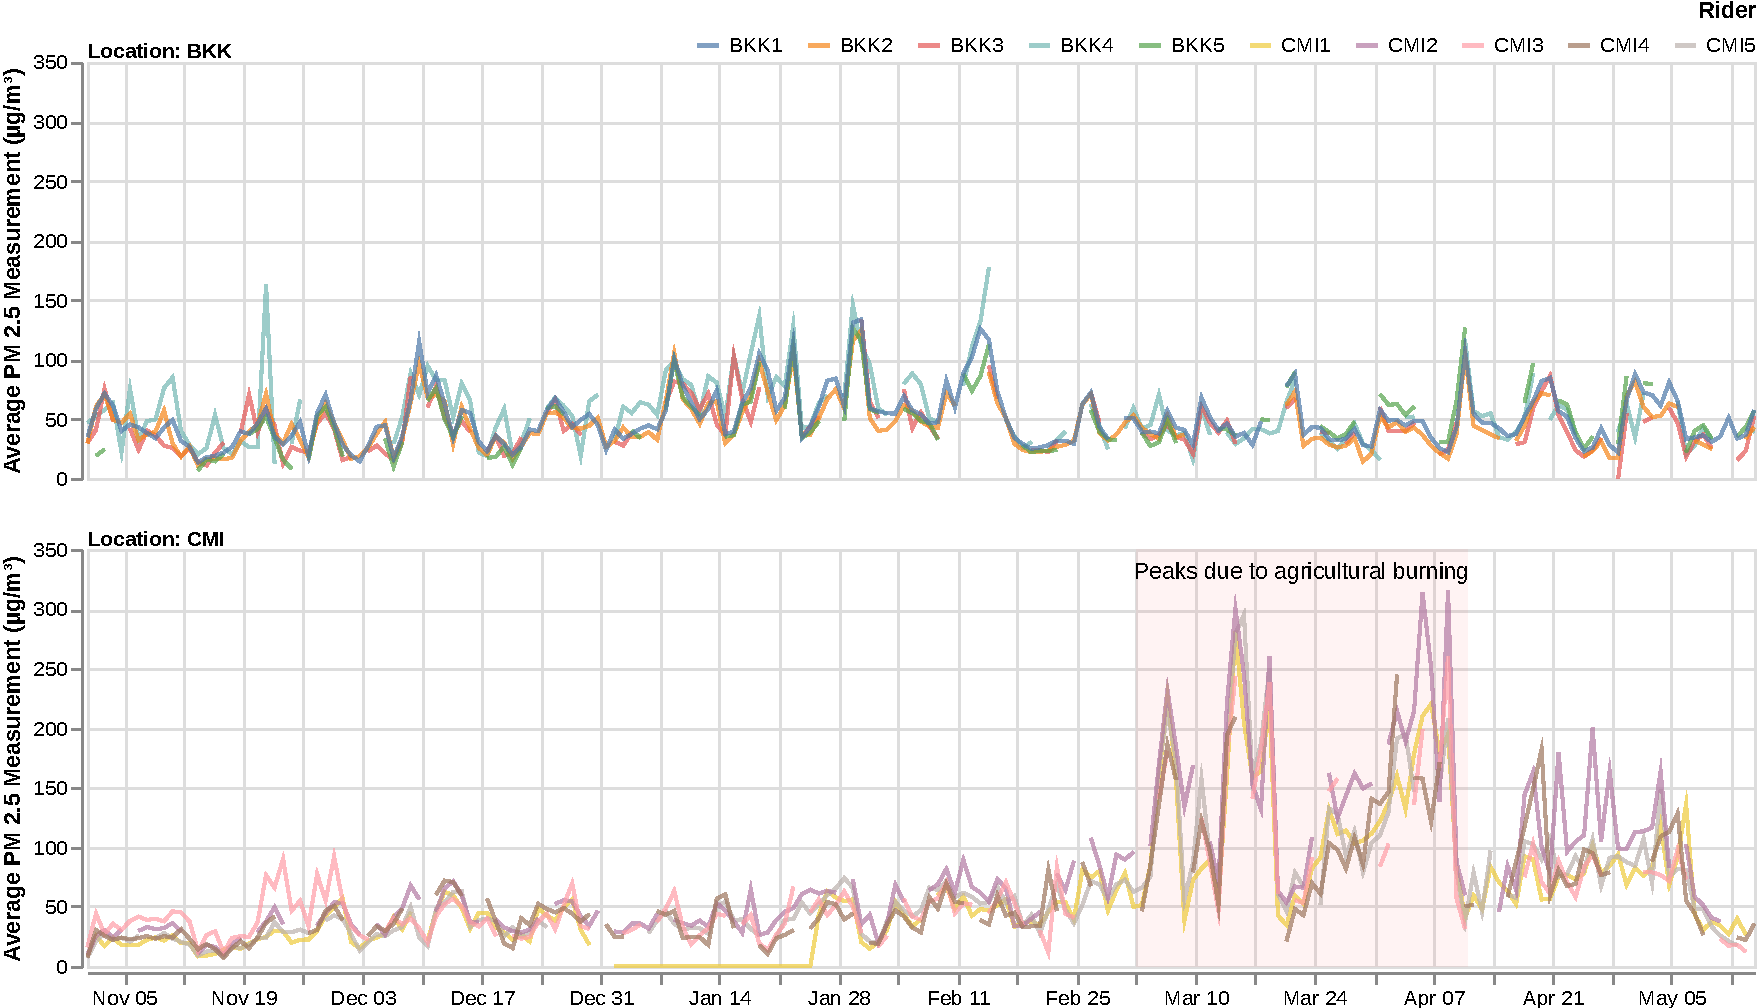
\includegraphics[width=\textwidth]{figures/daily-pollution-per-rider.pdf}
    \caption{
    Daily PM 2.5 exposure measured from the helmet-mounted sensors for Bangkok and Chiang Mai drivers.
    Vertical grid lines represent Sundays.
    }
    \Description{}
    \label{fig:daily-pollution-per-driver}
\end{figure*}

\subsection{PM2.5's Temporal Patterns}
Analyzing daily average PM2.5 exposure (\autoref{fig:daily-pollution-per-driver}) reveals relatively consistent levels in Bangkok (BKK), peaking moderately from December to mid-February,
while Chiang Mai (CMI) shows pronounced seasonality with extreme peaks from March to early April (consistent with agricultural burning periods~\cite{david2025chiangmaiburn, bernsten2024chiangmaiburn, iqair2023chiangmaiburn}).
% \joe{if you're going ot highlight it in the text like this, i would also highlight it in the figure}
Within each city, drivers experience similar daily trends.
Hourly averages (\autoref{fig:hourly-work-aqi}) show daily cycles peaking during morning (BKK: 7 AM, CMI: 8 AM) and evening rush hours, with an afternoon dip, although late night/early morning data shows higher variance.
Notably, BKK's PM2.5 measurements show a consistent trend throughout the year, reinforcing traffic as the primary air pollution source.
In contrast, CMI's dominant seasonal variation indicates agricultural burning as the primary driver.
Thus, PM2.5 sources differ substantially between cities (BKK: traffic, CMI: agricultural burning), implying the need for location-specific mitigation strategies.

% To find the PM 2.5 exposure amount of each driver throughout the different periods of the study,
% we present a relationship of the average amount of PM 2.5 measured from our sensor against days in the study in \autoref{fig:daily-pollution-per-driver}.
% We can see that the peak pollution in Bangkok is from December to mid-February; however, the amount of air pollution Bangkok drivers are exposed to is relatively consistent throughout the study period compared to that of Chiang Mai.
% On the other hand, PM 2.5 in Chiang Mai reaches high peaks from March to early April and low peaks afterward until May.
% We can attribute this consistency of the PM 2.5 level in Bangkok to its constant heavy traffic.
% In contrast, the condensed PM 2.5 peak period in Chiang Mai is consistent with yearly agricultural burning periods,
% which typically end in April,
% as evidenced by climate articles~\cite{david2025chiangmaiburn, bernsten2024chiangmaiburn, iqair2023chiangmaiburn}.
% % \mick{enforcement for agricultural burning}\footnote{\mick{\url{https://radiochiangmai.prd.go.th/th/content/category/detail/id/57/iid/352430}, \url{https://maesa.go.th/public/list/data/detail/id/5046/menu/1554}}}
% In addition, despite each driver's independence,
% all of the drivers in the study in each location still are exposed to the same amount of pollution, as shown in \autoref{fig:daily-pollution-per-driver}.

% To drill down into the finer-grain time period, we analyze PM 2.5 exposure patterns throughout each of the drivers' work days, as shown in \autoref{fig:hourly-work-aqi}.
% We can observe that the PM 2.5 exposure is consistently the highest at 7 AM for Bangkok and 8 AM for Chiang Mai, as these are both provinces' rush hours.
% The measurements for both provinces consistently slope down until the afternoon when they reach their lowest measurement values.
% The measurements climb back up again in the evening as workers travel back to their residents.
% The measurements collected at late night and early morning are inconsistent as indicated by the wider standard deviation range.
% % \mick{can we say here that because we have fewer data points -> less consistent?}
% The pattern with high PM 2.5 exposure during the morning and afternoon is less visible from March to May in Bangkok.
% This is the period when the majority of schools in Bangkok are on Summer break.
% The measured PM 2.5 patterns are highly correlated with Bangkok residents' commute behavior.
% This correlation further emphasizes that the primary source of PM 2.5 measured by Bangkok drivers is traffic pollution.
% On the other hand, in Chiang Mai, the measured PM 2.5 pattern with respect to months of the year is more prominent than patterns observed from measured PM 2.5 within a day.
% This indication leads us to conclude that the primary source of PM 2.5 measured by Chiang Mai drivers is agricultural burning.
% These results are also consistent with our analysis for \autoref{fig:daily-pollution-per-driver}.
% % \mick{can add analysis of PM 2.5 per day of the week if we have space.}

\begin{figure*}
    \centering
    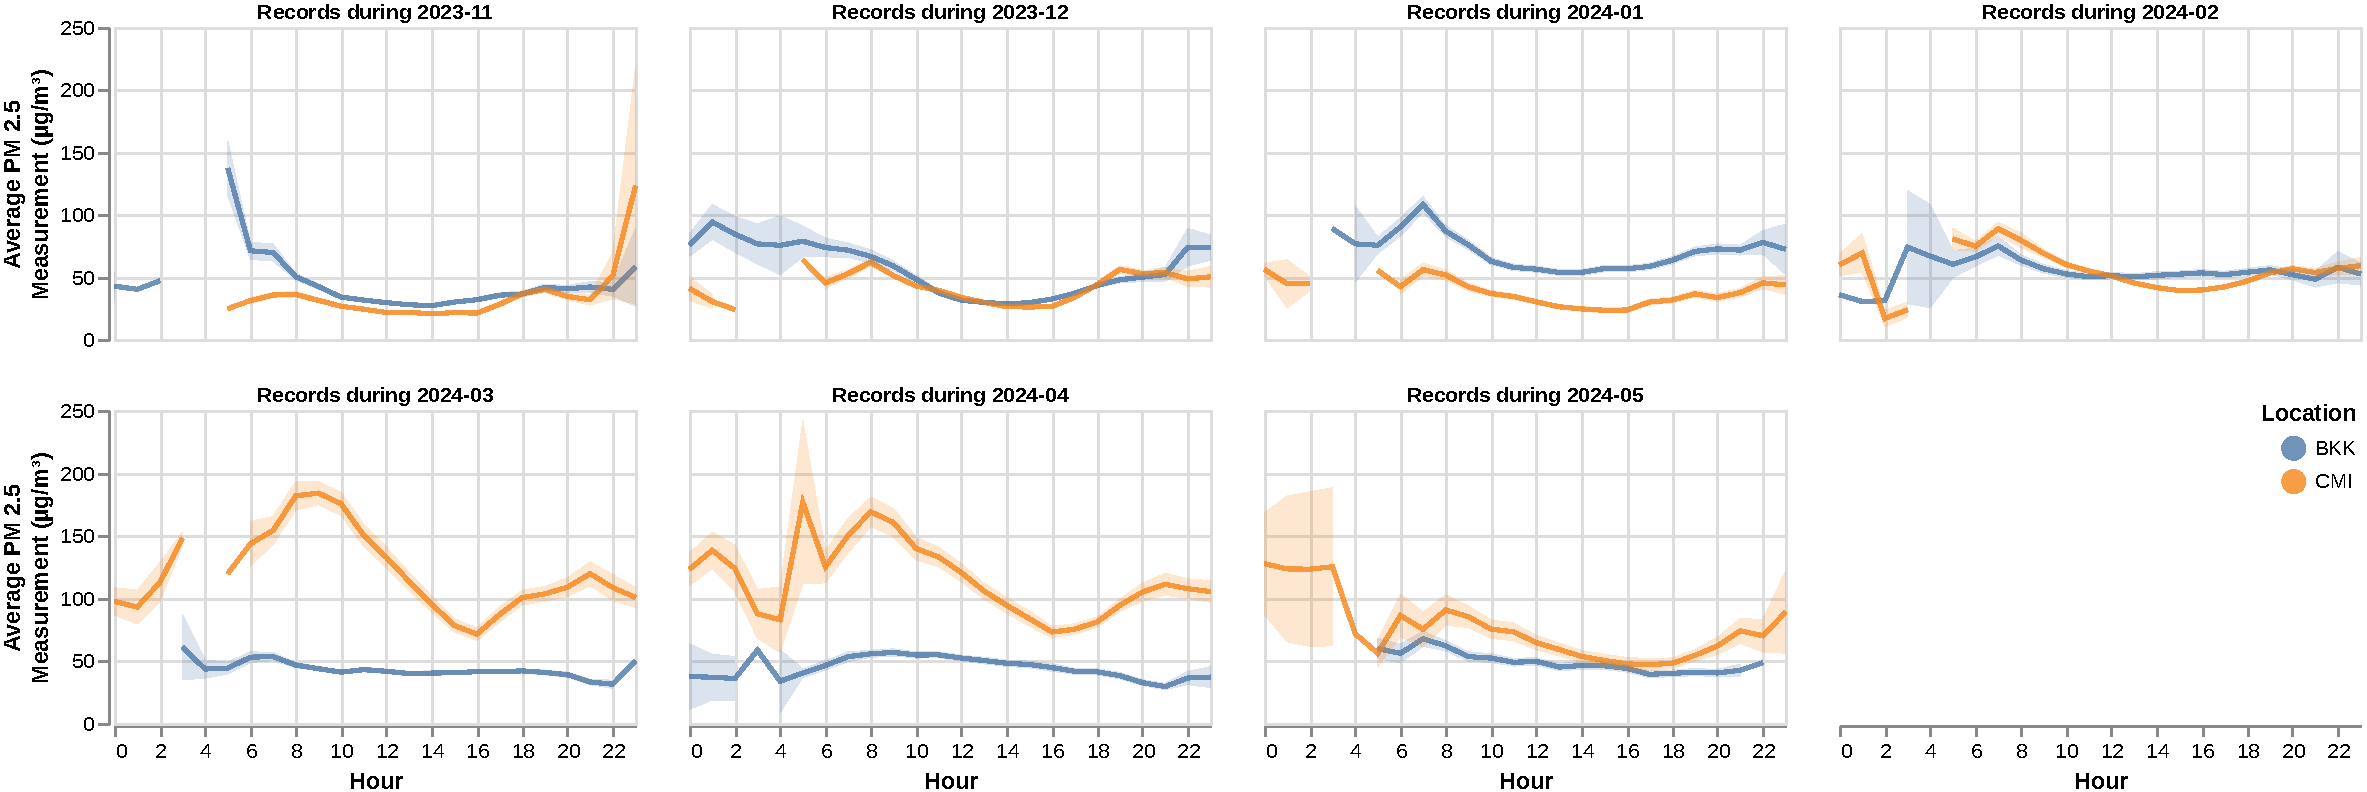
\includegraphics[width=\textwidth]{figures/average-hourly-pollution.pdf}%
    \caption{Mean and standard deviations of air pollution measurement in each hour of the day throughout the study period.
    % Each colored band represents $\pm1$ standard deviation from its average line. \joe{you can just say "mean and standard deviations shown" people know what fillbetween() represents.}
    Each subplot represents each month in the study. }%
    \Description{}
    \label{fig:hourly-work-aqi}%
\end{figure*}%

% % \begin{figure}
% %     \centering
% %     \begin{subfigure}[t]{0.49\textwidth}
% %         \centering
% %         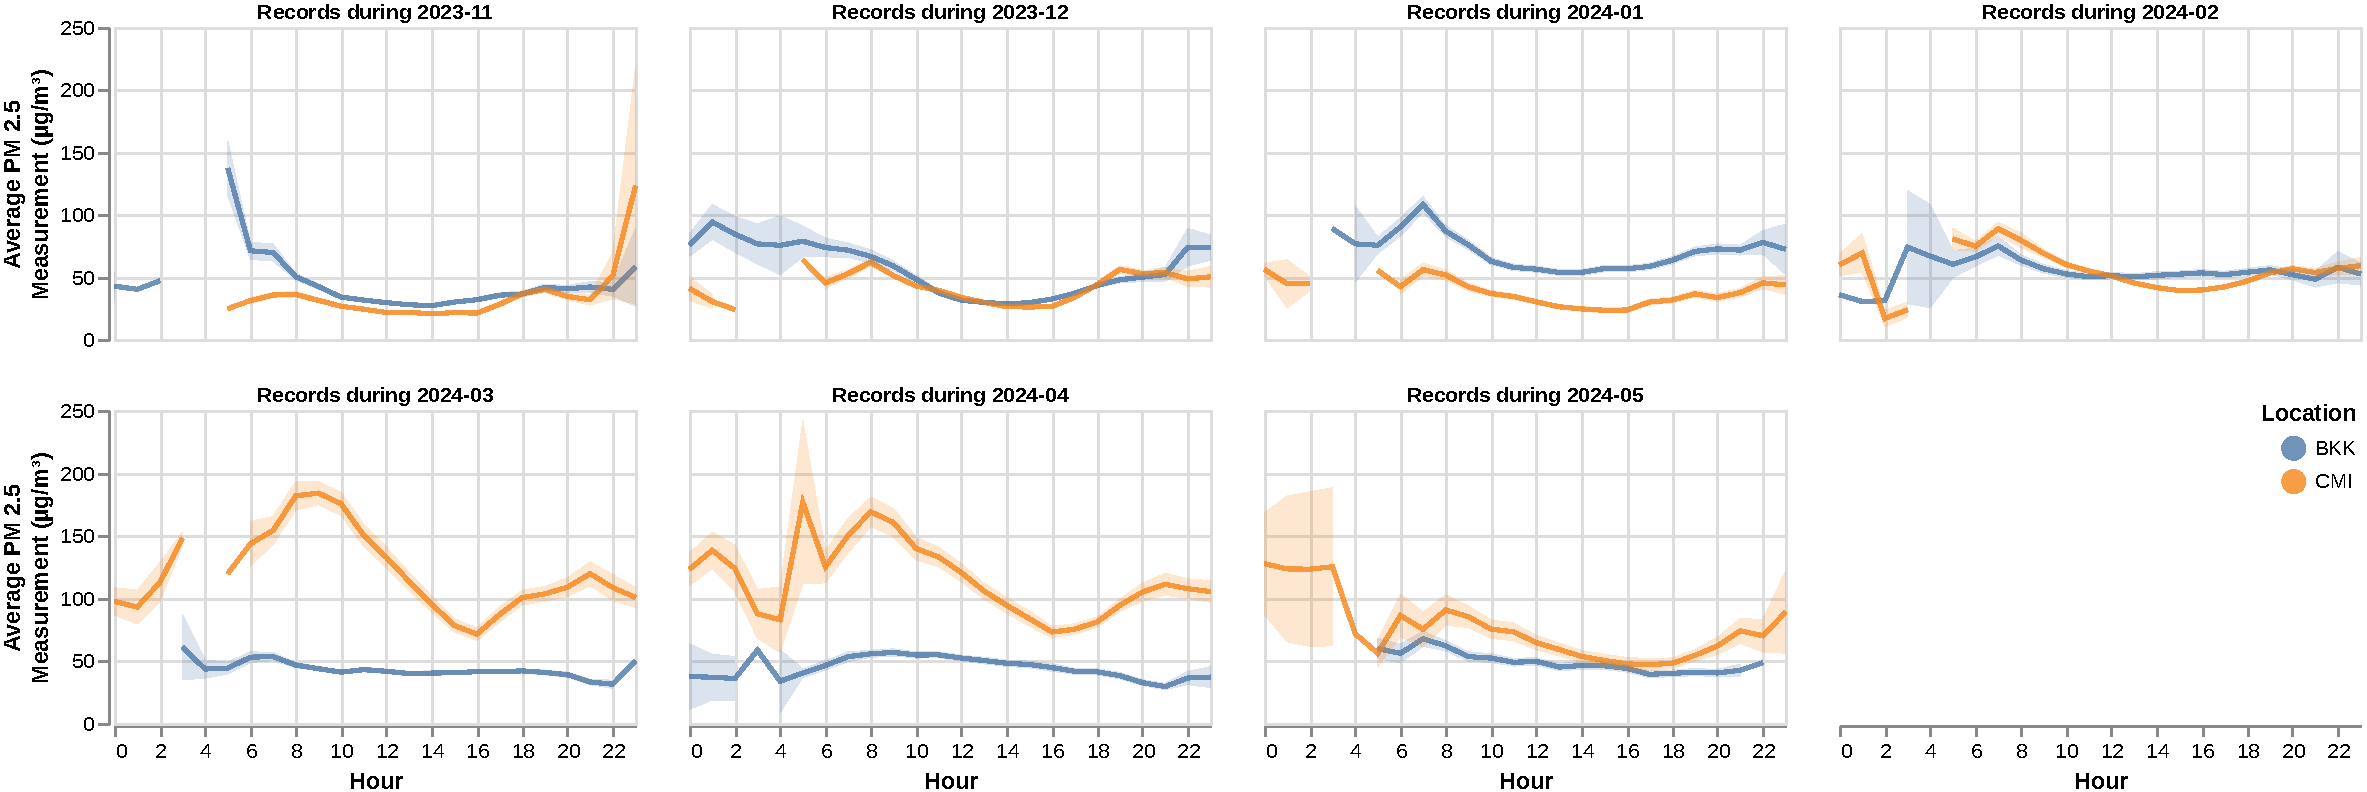
\includegraphics[width=\linewidth]{figures/average-hourly-pollution.pdf}%
% %         \caption{Average air pollution measurement in each hour of the day throughout the study period.}
% %         \label{fig:hourly-work-aqi}
% %     \end{subfigure}%
% %     \hfill%
% %     \begin{subfigure}[t]{0.49\textwidth}
% %         \centering
% %         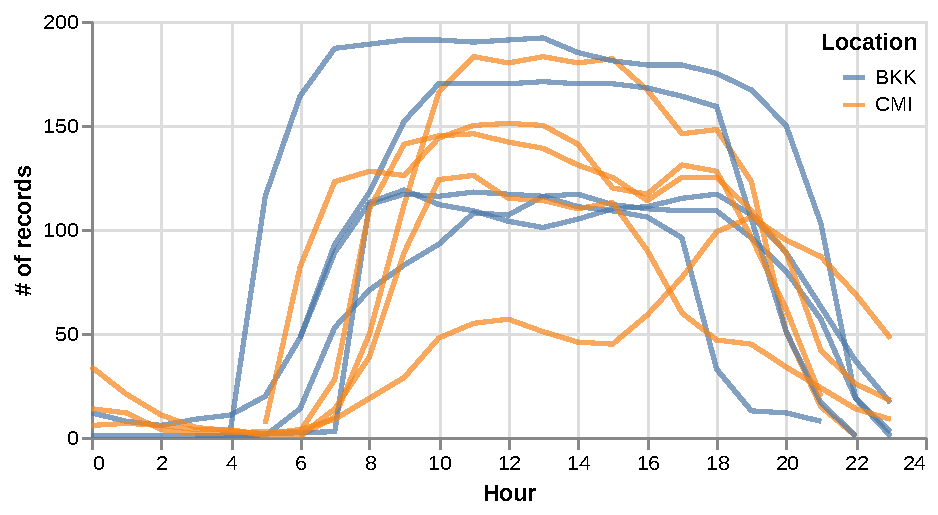
\includegraphics[width=\linewidth]{figures/hourly-records-per-location.pdf}%
% %         \caption{Number of records for each hour of the day throughout the study period. \mick{todo: divide by the \# of days they work}}
% %         \label{fig:hourly-work-hours}
% %     \end{subfigure}%
% %     \caption{
% %     Air pollution exposure and hour work for each hour of the day.
% %     \joe{shift x axis index by 1 so its not 0-23 but 1-24 for right plot and explain in text whether we actually have rider data from 22-3 as and how often. was it a few riders that drove at night?}
% %     }%
% %     \label{fig:hourly-work-stats}%
% % \end{figure}%

% % {\bf Answers to QS1.}
% \paragraph{Answers to QS1}
% % \mick{peaks at xxx; bkk is more consistent; chiang mai has lower pm 2.5 values during the normal period, but higher peaks; drivers seem to be exposed to similar amounts of PM 2.5 among drivers in the same province.}
% The PM 2.5 measured in Chiang Mai primarily follows the patterns of agricultural burning,
% while PM 2.5 measured in Bangkok primarily correlates with the commute behaviors of Bangkok residents and, thus, likely comes from traffic pollution.
% % \mick{the time granularity? for tackling AQ problem in each region are different (no one solution that fits regions)}
% As a result, the solution for lessening the amount of PM 2.5 exposed between both provinces must be different depending on the source of air pollution.

\subsection{PM2.5's Spatial Patterns}
% The results from analyzing the temporal patterns of PM 2.5 measurement indicate that participants in the same province are exposed to PM 2.5 at a similar amount at any given time throughout the study.
% In this section, we analyze the relationship between the amount of PM 2.5 measured and the locations of the drivers.
% As shown in \autoref{fig:subdistrict-aqi}, in each sub-figure, the plots in the right columns reveal that all of the drivers in the study mostly stay in one location. 
% The plots in the left columns also reveal that the PM 2.5 level is distributed unevenly across both provinces' subdistricts and drivers.

% \paragraph{Answer to QS2}
% The drivers experience different amounts of PM 2.5 even at the same approximate location.
% Each driver also spends the majority of their time at a different place.
% As a result, the solution for reducing the drivers' exposure to PM 2.5 should also take into account their active locations during their work.
Spatial analysis (\autoref{fig:subdistrict-aqi}) reveals that PM2.5 distribution is uneven across subdistricts and individual drivers, with drivers experiencing different exposure levels even in similar areas.
Furthermore, each driver tends to operate primarily within specific locations.
Consequently, effective PM2.5 exposure mitigation strategies must consider these individual spatial work patterns.
% \joe{is there openstreetmap in bangkok and chiangmai? can you compare the AQI with some environmental feature that you can pull from OSM? For example, number of intersections, width of roads, density of roads, etc. Would be cool to try to actually learn something about why AQI is worse in certain areas.}

\begin{figure*}
    \centering
    \begin{subfigure}[t]{0.49\textwidth}
        \centering
        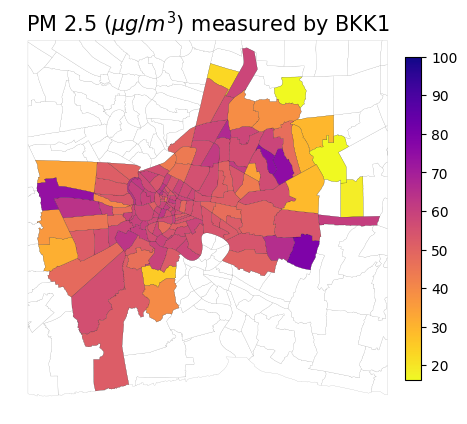
\includegraphics[width=.49\linewidth]{figures/map/BKK1_PM25.png}%
        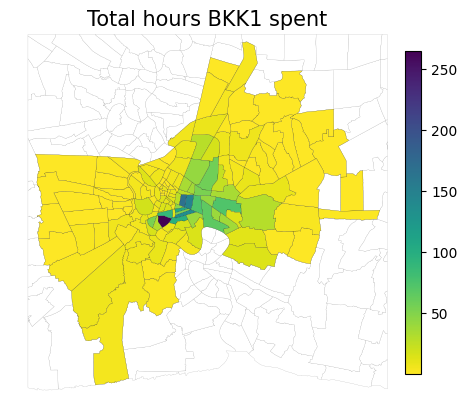
\includegraphics[width=.49\linewidth]{figures/map/BKK1_time.png}
        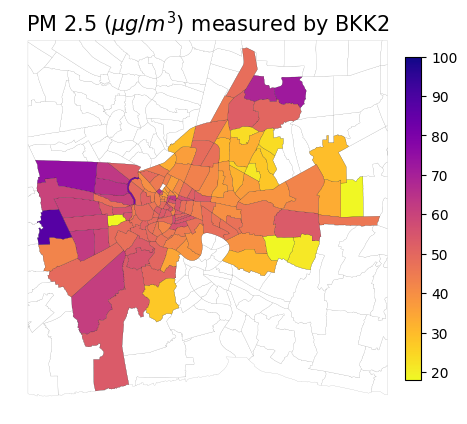
\includegraphics[width=.49\linewidth]{figures/map/BKK2_PM25.png}%
        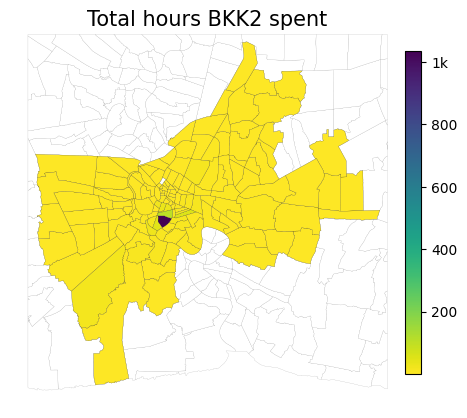
\includegraphics[width=.49\linewidth]{figures/map/BKK2_time.png}
        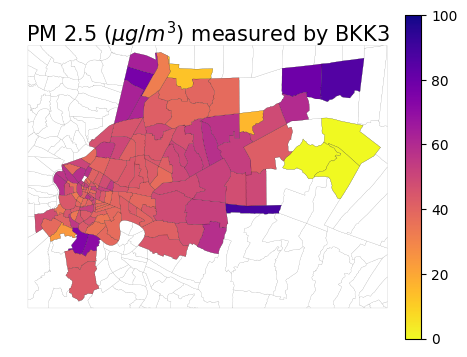
\includegraphics[width=.49\linewidth]{figures/map/BKK3_PM25.png}%
        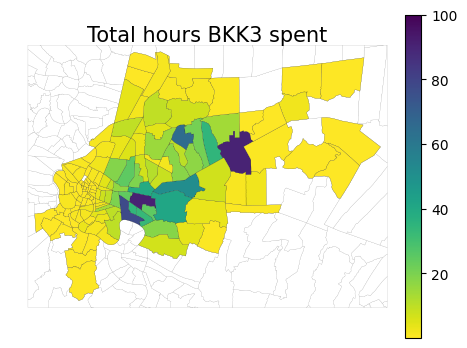
\includegraphics[width=.49\linewidth]{figures/map/BKK3_time.png}
        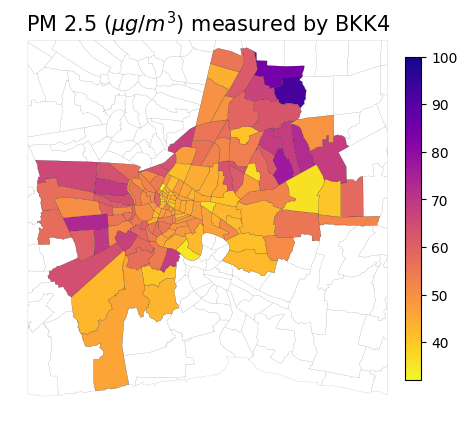
\includegraphics[width=.49\linewidth]{figures/map/BKK4_PM25.png}%
        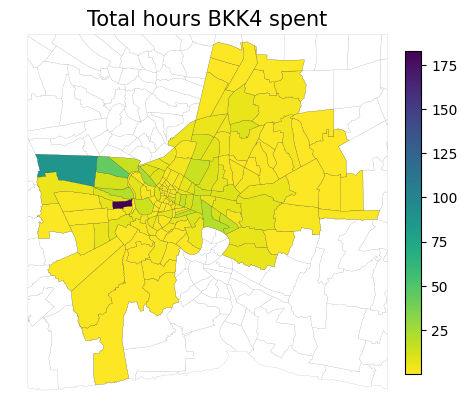
\includegraphics[width=.49\linewidth]{figures/map/BKK4_time.png}
        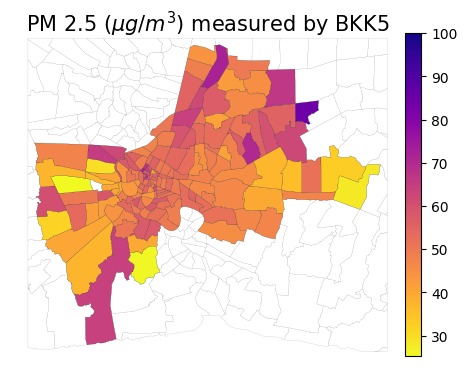
\includegraphics[width=.49\linewidth]{figures/map/BKK5_PM25.png}%
        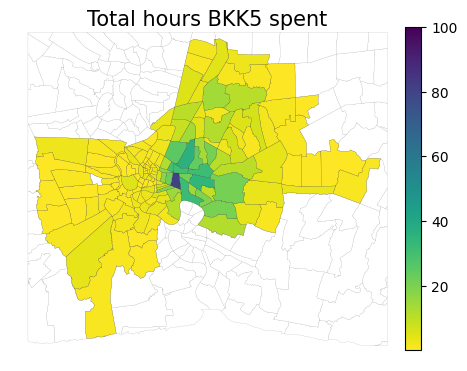
\includegraphics[width=.49\linewidth]{figures/map/BKK5_time.png}
        \caption{Measurement collected in Bangkok.}
        % \label{fig:hourly-work-aqi}
    \end{subfigure}%
    \hfill%
    \begin{subfigure}[t]{0.49\textwidth}
        \centering
        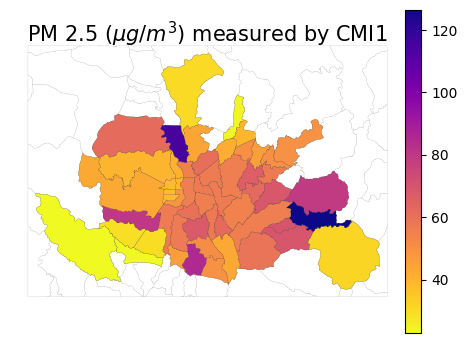
\includegraphics[width=.49\linewidth]{figures/map/CMI1_PM25.png}%
        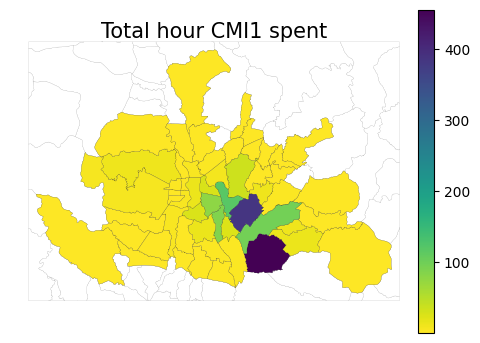
\includegraphics[width=.49\linewidth]{figures/map/CMI1_time.png}
        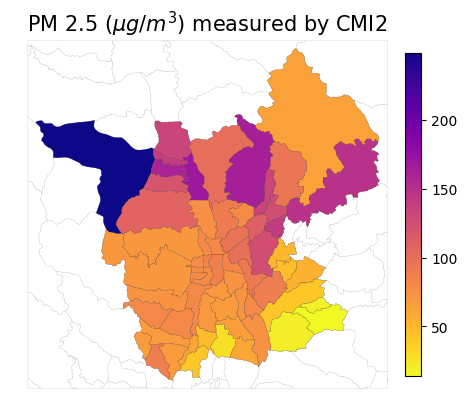
\includegraphics[width=.49\linewidth]{figures/map/CMI2_PM25.png}%
        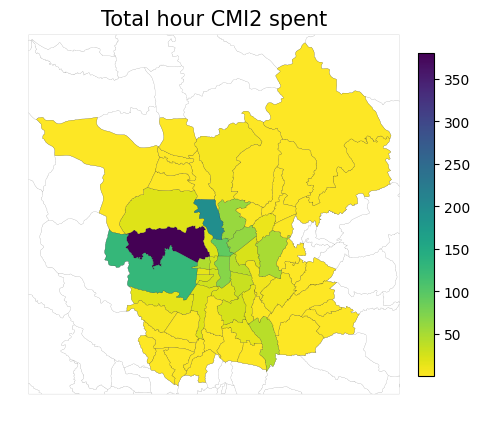
\includegraphics[width=.49\linewidth]{figures/map/CMI2_time.png}
        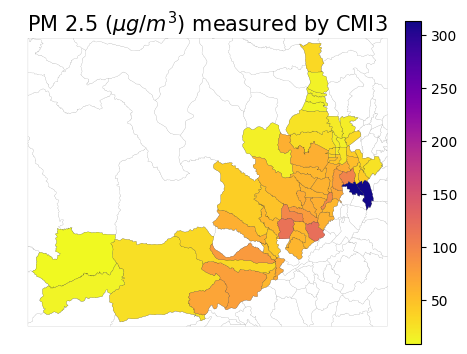
\includegraphics[width=.49\linewidth]{figures/map/CMI3_PM25.png}%
        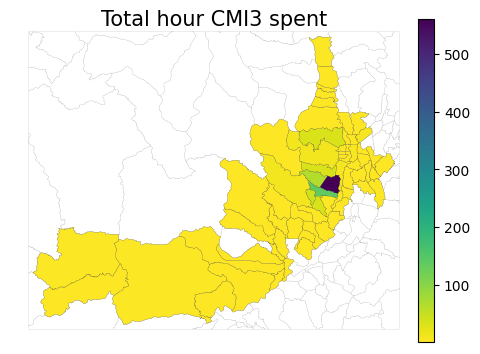
\includegraphics[width=.49\linewidth]{figures/map/CMI3_time.png}
        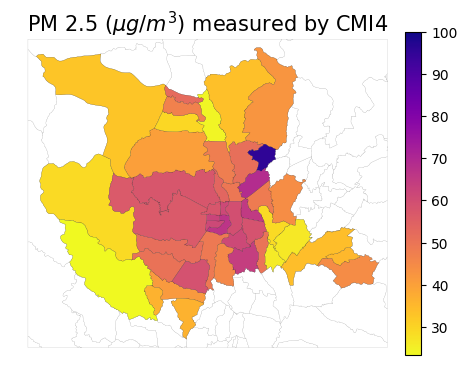
\includegraphics[width=.49\linewidth]{figures/map/CMI4_PM25.png}%
        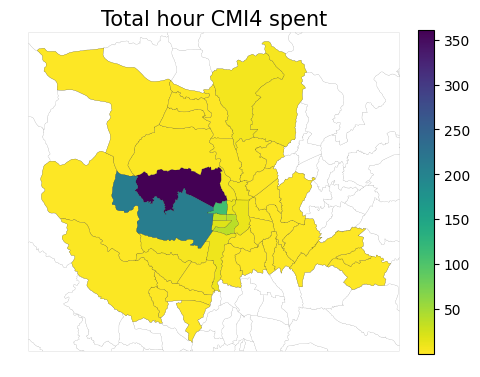
\includegraphics[width=.49\linewidth]{figures/map/CMI4_time.png}
        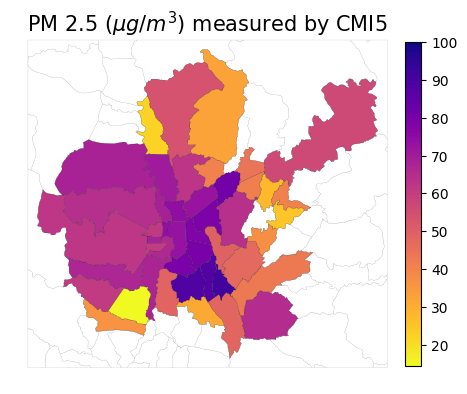
\includegraphics[width=.49\linewidth]{figures/map/CMI5_PM25.png}%
        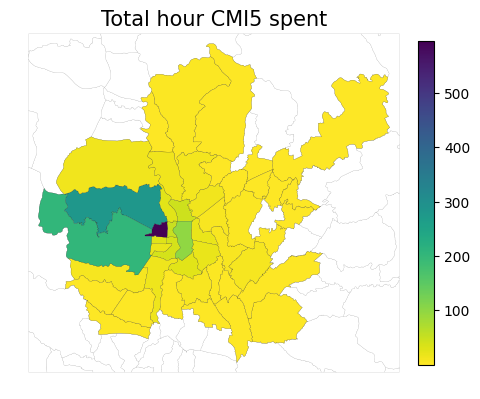
\includegraphics[width=.49\linewidth]{figures/map/CMI5_time.png}
        \caption{Measurement collected in Chiang Mai.}
        % \label{fig:hourly-work-hours}
    \end{subfigure}%
    \caption{
    % \joe{wait... the color bars are all wildly different on these plots lol. you can't even compare between them...}
    The left column of each sub-figure shows the average PM2.5 level throughout the study period measured in each subdistrict.
    The right column of each sub-figure shows the amount of time in hours that each driver spent in each subdistrict throughout the study.
    % \mick{todo: shared color axis?}
    % \mick{todo: same vis sizes}
    % \mick{todo: use latex notation for units}
    % \mick{todo: include all the subdistricts}
    % \joe{Shall we lower the opacity of the districts where there is no data at all in the left plots? based on the right plot, I can't tell if the purple districts have 0 hours spent or a very small amount of hours spent. If it is 0, I don't want to see measurements in the left plot. Maybe every person spent time in every district so if we want to make this more clear, just do a log plot in color dimension.}
    }%
    \Description{}
    \label{fig:subdistrict-aqi}%
\end{figure*}%

% \input{sections/4-2-systemic-3-response}
\subsection{Driver Responses to Air Pollution Exposure}
This section explores how drivers responded to the observed air pollution patterns, combining quantitative findings with qualitative insights from interviews and driver archetypes (``Income-Driven'' and ``Health-Conscious'').
While quantitative analysis reveals complex exposure patterns varying temporally (\autoref{fig:daily-pollution-per-driver}, \autoref{fig:hourly-work-aqi}) and spatially (\autoref{fig:subdistrict-aqi}) across individuals and cities,
driver responses show limited adaptation, dictated primarily by economic needs and the perceived unavoidability of pollution.

\subsubsection{Prioritizing Income Amidst Pervasive Pollution}
Our analysis reveals no correlation between drivers' daily work hours and concurrent average PM2.5 levels (\autoref{fig:work-hours-vs-aqi-per-rider}), indicating a lack of temporal work adjustments in response to pollution fluctuations.
This aligns with qualitative interviews where drivers frequently expressed perceiving pollution exposure as an unavoidable occupational hazard rather than a modifiable risk.
Many prioritized immediate income over avoiding polluted times, echoing sentiments like,

\qpadding
\fcolorbox{gray}{white}{%
  \begin{minipage}{.9\linewidth} \em
``I just go where the application tells me to go, ..., the (air) pollution is everywhere anyway.'' (BKK1)
  \end{minipage}
}

\qpadding
\fcolorbox{gray}{white}{%
  \begin{minipage}{.9\linewidth} \em
    ``When I see that the area gets smoggier, I often thought about driving out to the suburban area. But that means I'll have to drive an empty car out.'' (BKK5)
   \end{minipage}
}
\qpadding

This ``Income-Driven'' approach was common.
Driver BKK1 (46, Male), targeting 2,000-2,500 baht daily through long hours (4 AM-9 PM), exemplified this.
Despite experiencing symptoms like runny noses and eye irritation and becoming aware of pollution levels via our map visualization after joining the study, his driving patterns remained unchanged.
He explained his reliance on masks and persistence:

\qpadding
\fcolorbox{gray}{white}{%
  \begin{minipage}{.9\linewidth} \em
    ``I can feel my body gets weaker (the more I drive); I always wear masks. ... If Google Maps tells us to go, I go. Wherever it is, I just have to push through.'' (BKK1)
  \end{minipage}
}
\qpadding

He further emphasized the lack of choice dictated by the platform and financial needs:

\qpadding
\fcolorbox{gray}{white}{%
  \begin{minipage}{.9\linewidth} \em
    ``I will not be able to be selective about routes; I go wherever the application assigns me to go, no matter of how far or how polluted the area may be.'' (BKK1)
  \end{minipage}
}
\qpadding

% This practice, where enduring poor air is ``simply something they have to be able to live with'' (BKK-4), mirrors observations in gig work research regarding the normalization of health risks under precarious conditions.

% \begin{quoteb}
%     ``People who choose to become (motorcycle taxi) drivers, they know what they get themselves into. Pushing through rains or pollution is simply just something they have to be able to live with.'' (BKK-4)
% \end{quoteb}

% While drivers do not adjust work schedules, spatial analysis reveals they spend the majority of their time in subdistricts with relatively lower PM2.5 levels (below 100 $\mu g / m^3$, often below 50 $\mu g / m^3$).
% This suggests some passive or possibly active spatial avoidance, perhaps by choosing service areas known anecdotally to be less polluted, even if not actively avoiding specific high-pollution zones on a trip-by-trip basis.
The dominant narrative remains that immediate economic needs override pollution avoidance strategies concerning work timing.

\subsubsection{Limited Mitigation}
While prioritizing income was dominant, some drivers, exemplified by the ``Health-Conscious'' driver BKK3, attempted mitigation strategies within existing constraints.
BKK3 (54, Female) actively incorporated heightened air pollution awareness into driving decisions after using the sensor helmet and map visualization.
She observed pollution spikes when riding behind buses,

\qpadding
\fcolorbox{gray}{white}{%
  \begin{minipage}{.9\linewidth} \em
    ``When I follow big buses, the graph just shoots up immediately.'' (BKK3)
  \end{minipage}
}
\qpadding
% \begin{quoteb}
%     ``When I follow big buses, the graph just shoots up immediately.'' (BKK3)
% \end{quoteb}

and gained insight into hazardous AQI levels (80-100 \textmu{}g/m$^3$) even on seemingly clear days. This awareness prompted actions like avoiding main roads for side streets, despite potentially longer distances,

\qpadding
\fcolorbox{gray}{white}{%
  \begin{minipage}{.9\linewidth} \em
    ``Main roads have more dusts (air pollutants), it’s better to go through small alleys.'' (BKK3)
  \end{minipage}
}
\qpadding

and selectively accepting rides or disabling auto-matching nearby to reduce prolonged exposure, particularly when heading home.

% However, complete avoidance was impossible due to passenger demand and platform algorithms.
% Physical symptoms (nasal irritation, dry throat) sometimes led her to finish work early,
% \begin{quoteb}
%     ``I go home earlier quite often when I feel my nose stings and my throat feels dry.'' (BKK-3)
% \end{quoteb}

% Moreover, immediate safety threats like rain were prioritized over pollution concerns \cite{tieanklin2024rideshare}.
However, despite finding the real-time, localized AQI data useful, financial needs prevailed:

\qpadding
\fcolorbox{gray}{white}{%
  \begin{minipage}{.9\linewidth} \em
    ``We took this job for the money. We just have to live with it.'' (BKK3)
  \end{minipage}
}
\qpadding

BKK3's experience illustrates the tension between health awareness and economic necessity.
% , highlighting the limited scope for individual mitigation.
While information tools provide valuable insights, platform constraints significantly limit drivers' ability to act on this information without sacrificing income.

In this study, we do not observe a correlation between drivers' mitigation behaviors and their age or gender.

\subsubsection{Increased Awareness and Community Engagement}
Participation in the study and access to the map visualization significantly increased drivers' awareness and spurred public engagement.
Most participants reported frequently checking the visualization, particularly on high-pollution days.
This led to discussions about air quality with friends and passengers; for instance, CMI4 advised others on mask use, while BKK4 shared real-time data from the visualization with passengers during rides in poor conditions.
The visualization thus served both as a personal reference tool and a catalyst for community awareness.

Driver CMI1 exemplified proactive community engagement.
He monitored morning pollution levels and actively shared warnings in the Chiang Mai rideshare driver community (>5,000 members) when conditions were hazardous:

\qpadding
\fcolorbox{gray}{white}{%
  \begin{minipage}{.9\linewidth} \em
 ``I often take a screenshot (of the map visualization) when the air pollution levels turn red (hazardous) and share it in the group, warning everyone to be extra careful since the pollution got worsen that day.'' (CMI1)
  \end{minipage}
}
\qpadding

This demonstrates how access to real-time, localized data empowered drivers beyond personal monitoring.
It fostered collective awareness and turned some participants, like CMI1, into informal educators and active contributors to environmental health knowledge sharing within their community, moving beyond passive data reception.

\begin{figure*}
    \centering
    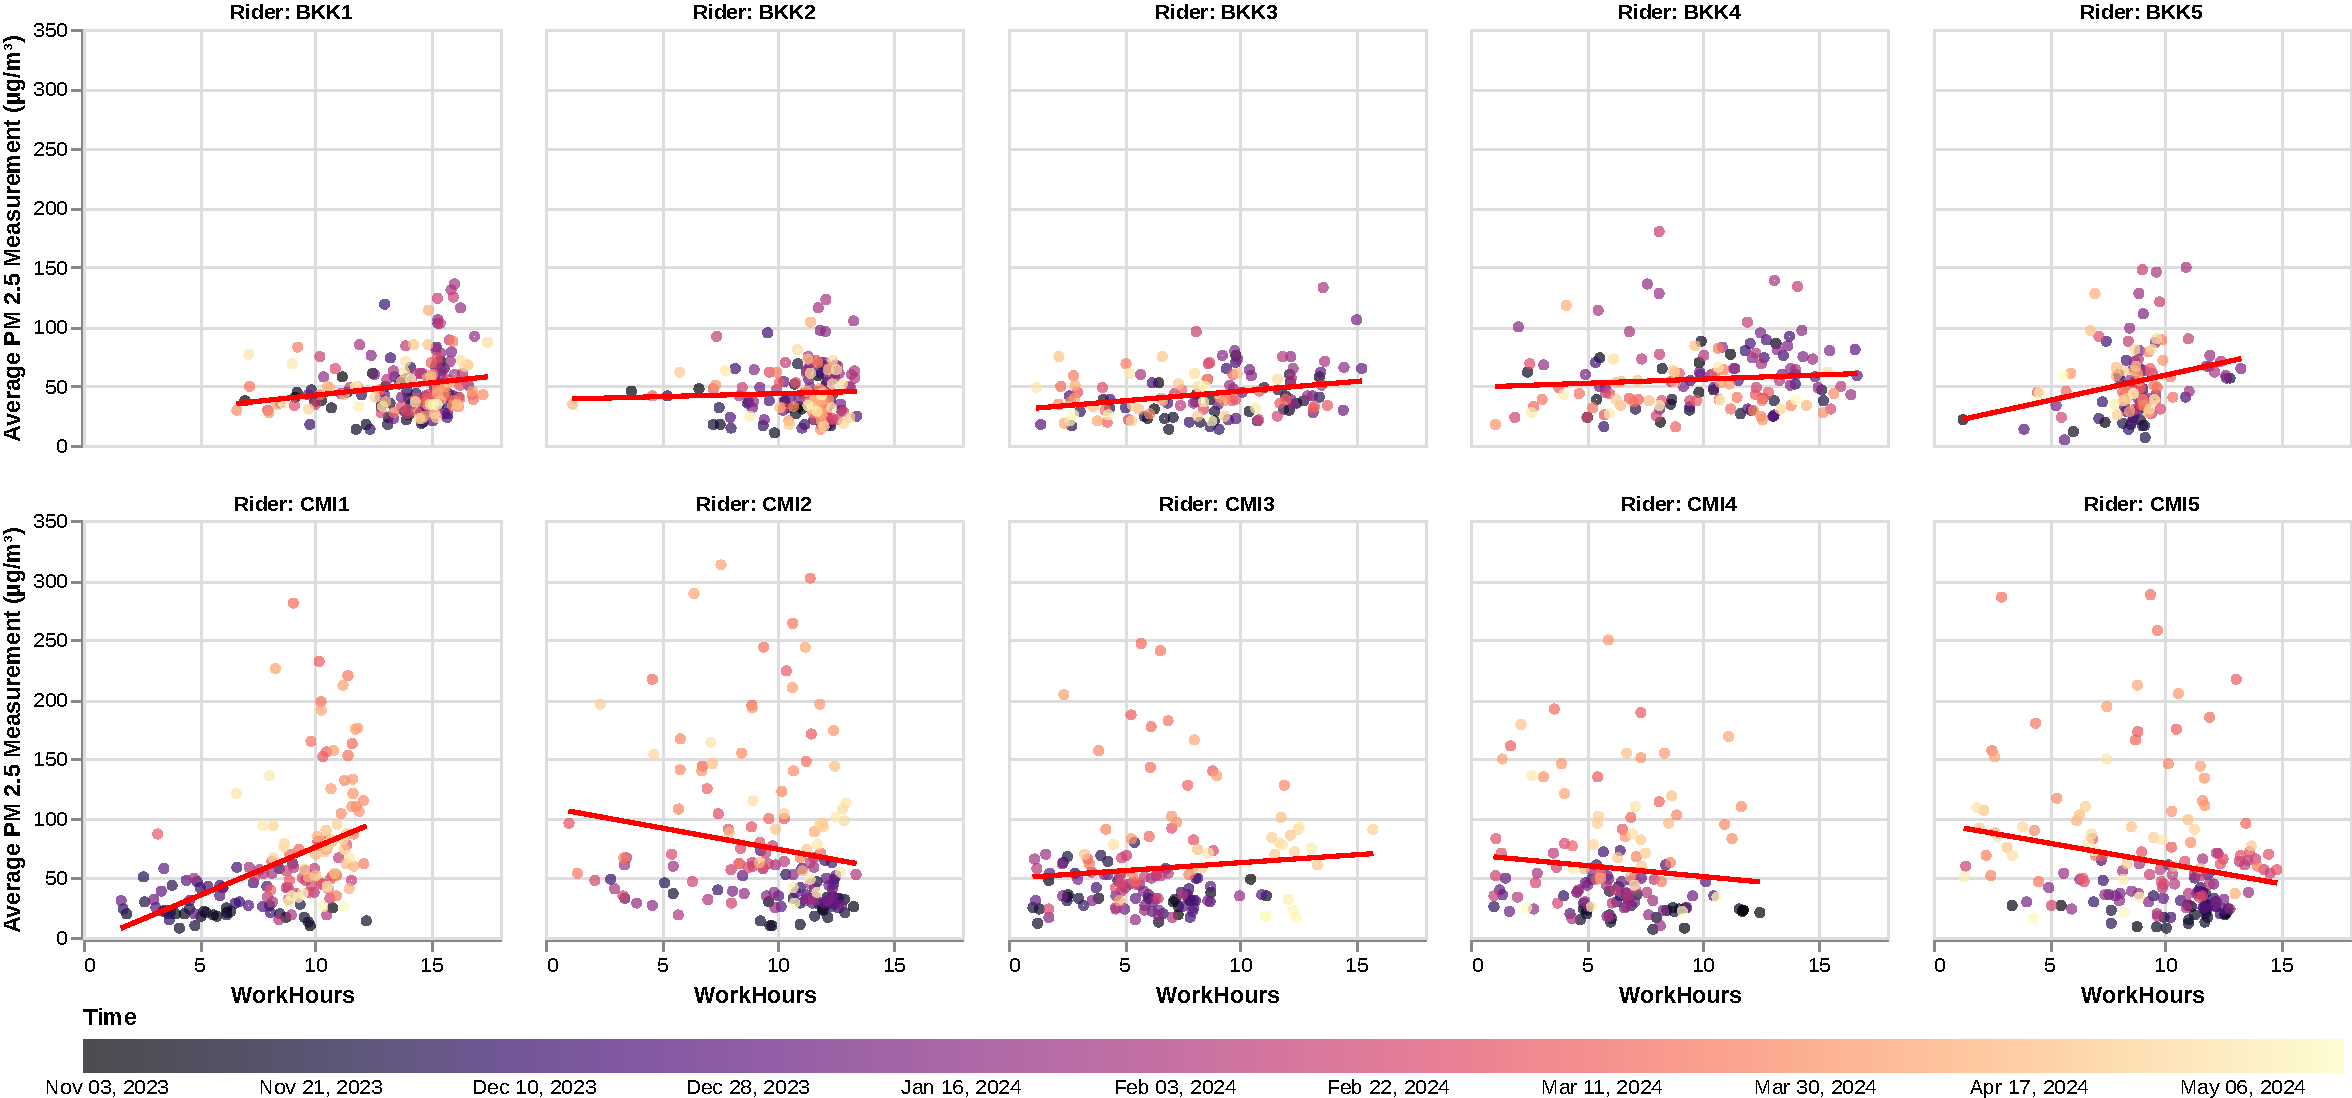
\includegraphics[width=\textwidth]{figures/work-hours-vs-aqi-per-rider-regression.pdf}
    \caption{Correlation of daily work hours and air pollution measurement for each driver, averaged through each week, with regression lines.
    % \joe{why are we aggregating to a weekly scale if we have daily data? A scatterplot is literally the perfect opportunity to represent disaggregated data and based on the fact that so many plots in this paper are per-participant, it seems like you wnat to show as fine grained data as possible?}
    }
    \Description{}
    \label{fig:work-hours-vs-aqi-per-rider}
\end{figure*}

Overall, while access to air quality information increased awareness and even spurred community engagement, the demanding nature of gig work and the perceived ubiquity of pollution limit drivers' capacity to translate this awareness into significant behavioral changes, particularly regarding work schedules.
Financial imperatives largely override health considerations, highlighting the need for systemic interventions beyond individual information provision to effectively reduce exposure, such as low-emission zones or integrating real-time AQ data into traffic management.
% \input{sections/4-3-individual}
% \subsection{Communal Engagement -- From Technical Support to a Community Space}
\label{sec:result-communal-engagement}
% Group Interactions and Air Quality Discourse

In this subsection, we explore how motorcycle taxi drivers in Bangkok and Chiang Mai engaged in collective sensemaking through their group chat interactions, leveraging air quality data from their sensors. 

\subsubsection{Sense of Community and Social Support}
Initially created as a technical support channel, the group chat quickly evolved into a vital community space where drivers from both provinces, Bangkok and Chiang Mai, shared their day-to-day driving experiences, unexpected circumstances, traffic congestion and most importantly, warned each other about worsening air pollution conditions in their respective areas.  

During peak pollution days, the chat became particularly active, with drivers providing real-time updates. On December 11, 2024, one of the first major pollution waves of the season in Bangkok, driver BKK-5 began their day by checking the air quality web portal that we provided and alerting everyone in the groupchat,

\begin{quoteb}
    ``Today the air pollution is really thick, it's very red.'' (BKK-5)
\end{quoteb}

\mick{can remove this paragraph because does not make the point for the communal engagement.}
BKK-5 Driver also reported during the exit interview that he often checked the map visualization showing the air pollution level every day and constantly checked for updates throughout the day, especially during the peak period in January and February.

Beyond leveraging the data that they have collectively collected, the group chat functioned as a space for social support, where drivers expressed concerns about health risks and reminded other participants, sometimes the research team included, to prepare protective measures mitigating exposure. 
This illustrates how the integration of sensor data into social communication channels can enhance risk awareness and foster a sense of community among participants.


\subsubsection{Shared Situational Awareness and Collaborative Interpretation}
Beyond warnings, drivers also used the visualization tools to compare pollution levels between the two cities, Bangkok and Chiang Mai, fostering a shared understanding of exposure risks. 
% Some expressed concerns about their peers’ conditions, reinforcing a sense of solidarity despite being geographically apart.
Our participants reported developing a new habit of frequently checking both their own and other participants' air quality measurements using the map visualization web application, particularly during downtime while waiting for the next ride request.
For instance, BKK-4 was the first to notice the onset of one of the worst air pollution waves in Chiang Mai of 2024, where sensor data showed PM2.5 levels exceeding 200 $\mu g/m^3$ during the day. BKK-4 remarked,

\begin{quoteb}
``(Air pollution in) Chiang Mai has been getting a lot worse a lot lately.'' (BKK-4)
\end{quoteb}

Drivers often use the visualization web application not only to navigate their immediate environment but also to stay informed about broader regional trends.

This emergent community dynamic highlights that drivers are not indifferent to air pollution risks; rather, as discussed earlier, they perceive it as an unavoidable part of their job. Given that motorcycle taxi driving is their primary source of income, individual avoidance strategies remain limited, further underscoring the need for broader structural interventions. 

\subsubsection{Leverage The Tool for Income}
Drivers frequently utilize the air quality map to identify ``red'' zones, which indicate high pollution levels, and infer traffic congestion in those areas. This capability allows them to strategize their routes to maximize income by avoiding congested areas while simultaneously minimizing exposure to poor air quality. 
The interviews with drivers have revealed the dual benefits of using the map visualization web application - optimizing income by increasing the number of pickups while also subsequently  reducing the health risks from the air pollutions as they would just avoid the area.
For instance, one of the most-earning Bangkok drivers noted during the exit interview,

\begin{quoteb}
``It will actually be even more helpful to actually show the traffic real-time, so I can avoid the area altogether...  I can make more rounds of pickups and also reduce the air pollution intake too.'' (BKK-5)
\end{quoteb}


The drivers’ ability to interpret air quality data in conjunction with traffic conditions reflects a strategic approach to their work, where financial incentives take precedence over health considerations. 
This aligns with the previous research for this particular group indicating that gig workers often prioritize immediate income due to precarious employment conditions, leading them to overlook long-term health implications \cite{tieanklin2024rideshare, zhang2022algorithmic}. 
This underscores the need for targeted interventions that address both economic and health concerns for gig workers in urban environments.
\section{Discussion}

This study combines sensor data and interviews to offer a multi-modal perspective on Thai motorcycle rideshare drivers' experiences.
A key goal was understanding this environment to identify interventions improving driver health and livelihoods.
We discuss driver interest in real-time data, policy implications, infrastructure improvements, and platform-level incentives.

\todo{what specific interventions-technological, regulatory, or organizational-do drivers themselves propose or prefer?}

\todo{How feasible are sensor-based early warning systems or adaptive work scheduling in practice?}

\todo{Are there gendered or age-related differences in exposure or agency?}

\para{User Interest in Real-Time Data}
Despite prior work~\cite{tieanklin2024rideshare} suggesting drivers prioritize revenue over technology-led behavioral change, participants valued real-time air quality data, feeling it empowered more informed decisions and increased awareness.
Drivers suggested integrating this data via motorcycle dashboards, ride-share apps, interactive maps, or directly into motorcycles.
Predictive algorithms could offer proactive warnings.
While designing non-distracting interfaces is challenging, this area warrants future investigation.


\para{Policy Interventions and Financial Support}
Government interventions like targeted financial support (e.g., subsidies for protective equipment, healthcare benefits, compensation during severe pollution) could improve driver outcomes.
Stricter emission controls and encouraging electric motorcycles offer long-term improvements.
Ultimately, reducing driver exposure requires a multi-stakeholder approach involving government, platforms, passengers, and drivers, integrating technology and policy to balance stakeholder needs (platform profitability, driver health/income, user convenience).

\para{Local and Collective Action}
The differing primary PM2.5 sources were identified; consistent traffic emissions in Bangkok versus seasonal agricultural burning dominating in Chiang Mai. 
This fundamentally shapes the air pollution challenge across regions and underscores that effective mitigation strategies must be location-specific. 
For instance, government policies like Work-From-Home (WFH) campaigns (e.g., Bangkok's 2024 initiative contributed to an 8\% traffic reduction  \cite{Wipatayotin_2025}) directly target the traffic congestion identified as Bangkok's primary issue, particularly during peak rush hours indicated by daily cycles (\autoref{fig:hourly-work-aqi}). 
Yet, these policies offer limited impact where sources differ (e.g., Chiangmai's burning season) and fail to resolve direct exposure for frontline workers like motorcycle taxi drivers who remain operational amidst pollution sources.
Therefore, effective solutions need integrated approaches by complementing national policies with targeted, local actions against dominant sources (traffic/burning) plus direct support (e.g., PPE, technology) for those highly exposed, potentially scaled through tailored public-private partnerships.






\para{Passenger Awareness and Platform-Level Incentives}
Ride-share platforms involve competing passenger and driver incentives.
For example, passenger demand for food deliveries during high pollution increases driver exposure.
Educating passengers about these risks could help.
Platforms could offer off-peak discounts during high-pollution events, aligning incentives, though potentially reducing platform usage.
Alternatively, external campaigns could discourage peak-pollution usage.








\para{Study Limitations}
Limitations include the sensor's battery power (8-10 hours), potentially causing data gaps during longer shifts despite recharge encouragement; direct motorcycle power is a future consideration.
Our non-random sample intentionally focused on uniquely deep, longitudinal lived experiences rather than generating statistically generalizable health conclusions typical of epidemiological studies.
Furthermore, sensors measured only a subset of pollutants, likely underestimating total exposure risks.

\section{Conclusion}

This study investigated the severe PM2.5 exposure faced by motorcycle rideshare drivers in urban Thailand, 
highlighting how economic constraints create significant barriers for this population to follow standard health advice, even when aware of the dangers.
Building upon previously identified agency limitations, our seven-month mixed-methods study uniquely introduced a real-time air quality map visualization,
observing that although drivers incorporated this data to adjust routes and schedules,
income generation consistently superseded significant exposure mitigation actions.

Our contributions include fine-grained, individualized exposure data contextualized by lived experiences, revealing the complex interplay between health risks, economic pressures, and structural barriers.
The findings underscore the urgent need for multi-faceted interventions involving technology (e.g., real-time data interfaces), policy (e.g., financial support, targeted regulations), and platform adjustments.

%%
%% The acknowledgments section is defined using the "acks" environment
%% (and NOT an unnumbered section). This ensures the proper
%% identification of the section in the article metadata, and the
%% consistent spelling of the heading.
% \begin{acks}
% \end{acks}

%  ccs concepts of mobile sensing, mixed methods, maybe applications in health? 

% Keywords: air quality sensing, mobile sensing, empirical analysis, etc. 

\begin{acks}
We thank the anonymous reviewers for their helpful feedback. 
This work was funded in part by the National Science Foundation (NSF) under Award No. 2025022. The findings and conclusions expressed are those of the authors and do not necessarily reflect the views of the NSF.
\end{acks}


%%
%% The next two lines define the bibliography style to be used, and
%% the bibliography file.
\bibliographystyle{ACM-Reference-Format}
\bibliography{references}

% \input{sections/8-appendix}
% \clearpage
\section*{COMPASS Reviews}
\subsection{Review \#45A}
\begin{table}[h]
\begin{tabular}{|l|l|}
    \hline
    \textbf{Overall merit.} &
    2. Weak reject \\
    \hline
    \textbf{Reviewer expertise.} &
    2. Some familiarity \\
    \hline
    \textbf{Paper Relevance to COMPASS} &
    1. Very relevant \\
    \hline
\end{tabular}
\end{table}

\paragraph{Summary}
The study deploys air quality sensor to their understand PM2.5 exposure for low-income motorcycle taxi drivers in Thailand. The core contribution of the work is to improve the level of awareness to the people, most exposed to the air pollution, by providing real-time monitoring. The study focuses on collecting data from helmet mounted air quality sensor for all the riders with an intention to help avoid exposure to air pollution. The study also analyzes the data and conducted interviews with the participants to gauge the impact of the deployment.

\paragraph{Strengths}
\begin{itemize}
\item 
The study performs both quantitative and qualitative analysis of the data regarding the PM2.5 exposure. Results show that although overall exposure doesn’t change, the awareness among the participants helped make changes to their driving pattern to avoid exposure.
\item
The study finds that socio-economic factors are a major hurdle in making changes to driving behaviors.
\end{itemize}

\paragraph{Weakness}
\begin{itemize}
\item
I am unsure of potential impact of this approach. Since pollution is everywhere, changing the route of the rider doesn't affect that much as admitted by some of the participants .
Also, the changing the route depends heavily on the economic factors and incentive from the platform as highlighted by the study. This makes me think whether the nuances which authors claim to be the core contribution are actually feasible in real-world when monitoring air quality.
\mick{In discussion: better policy for the solution?}
\item
The dataset is too small to draw any conclusions drawn here. I think work from [7] does a good job though in terms of number of participants. I think the authors need to be at least somewhat close to that.   
\mick{Our dataset is larger. We have 10 sensors, while they have 6. They have 400 participants for their survey, but we did months-long study.}
\item
The paper was difficult to understand and unnecessarily long which made it difficult to follow. The authors need to do better framing of the problem. The writing needs to be improved significantly.
\mick{We might want to cut the parts on emotional aspects of the participants (and maybe community building). Then, we can have a clearer objective of how to help drivers make healthier decisions without income tradeoffs.}
\end{itemize}


\clearpage
\subsection{Review \#45B}
\begin{table}[h]
\begin{tabular}{|l|l|}
    \hline
    \textbf{Overall merit.} &
1. Reject \\
    \hline
    \textbf{Reviewer expertise.} &
4. Expert \\
    \hline
    \textbf{Paper Relevance to COMPASS} &
2. Relevant \\
    \hline
\end{tabular}
\end{table}

This paper presents a study about motorcycle taxi drivers in Thailand using helmet mounted sensors to monitor their exposure to pm2.5. Using the sensor values and findings from qualitative studies that focus on user experience with the sensors and the data platform, the authors present results on times and locations with highest pollution plus the social implications of having access to air quality data.

\paragraph{Strengths}
\begin{itemize}
\item
the findings around the social uses of the data, including across cities and changing driver patterns is interesting and shows the potential of data access
\item
the interview coding section is nicely detailed
\item
the stated contributions are well laid out
\end{itemize}

\paragraph{Areas of opportunity}
\begin{itemize}
\item
the abstract is missing from the paper
\mick{fixed}
\item
the introduction is too short and does not properly introduce the problem (air pollution) and motivation behind this work. It should read like a summary of the paper to help guide the reader but is missing a lot of information
\item
the related works feel more like a critique of a few prior studies rather than an engagement with literature. I’d like to know 1) why the chosen topics are relevant to this work and 2) how this work fills a gap that emerges from prior work. I also don’t think the comparison to a paper about global poverty versus air pollution is the right one to make here \todo{Firn is at this}
\item
it also just feels like there needs to be more examination into prior work overall. The authors should compare to other mobile sensor studies, and be sure to indicate works they are referencing, i.e.  in section 5.1 
\item
I don’t understand the proposal of discounts during high pollution times mentioned in section 5.4. It seems this would just expose drivers to more pollution 
\item
I’m not sure I understand the point of figure 4. Its also confusing that it is referenced after figure 5 in the text so I don’t know if that is a textual error \todo{Mick is at this}
\item 
table 1 is not really demographic information, more employment information
\item
the authors state “ This results indicate that drivers choose their service location in a way that avoid locations with high PM 2.5 levels.” In response to qs2, but this seems at odds with the prior quote that said drivers just go where they need to
\end{itemize}

\paragraph{Minor}
\begin{itemize}
\item
typos throughout
\item
one sentence that says “exposure…??”
\item
starting a related works section with “this work” but that refers to a prior work that hadn’t been introduced yet
\item
unanonymized institution for IRB
\end{itemize}

Overall, I like the goals of this paper but feels that it needs a lot more work to be ready for publication. I hope the authors will take time to revise and make this feel like a full paper that lives up to its stated contributions then submit again.


\clearpage
\subsection{Review \#45C}
\begin{table}[h]
\begin{tabular}{|l|l|}
    \hline
    \textbf{Overall merit.} &
3. Weak accept \\
    \hline
    \textbf{Reviewer expertise.} &
2. Some familiarity \\
    \hline
    \textbf{Paper Relevance to COMPASS} &
3. Somewhat relevant \\
    \hline
\end{tabular}
\end{table}

This paper discusses a study run over seven months with motorcycle rideshare drivers in Thailand using a helmet-mounted air quality sensor. The paper discusses the findings from the study in a mixed methods approach, showing quantitative data of air quality alongside qualitative interview data.

The study is relevant to COMPASS, I believe, but perhaps doesn't quite address an HCI audience as we would hope.

I think this study is rigorous and very interesting. I loved seeing the people make sense of data and make decisions (or not) using this new information. I think the length of time and quantity of people surveyed, as well as the compensation for the study, are all commendable. I also found the detailed insights in the findings section fascinating and rich. As a qualitative researcher, I was less intrigued by the quant findings (although they do help tell a story of the rhythms of the seasons and days) – and was really invested in section 4.3 which was a wonderful ethnographic look at different ways of encountering this air quality data.

I feel a bit lost as to who the audience is and this is evident in the shaping and framing of the paper and the discussion and take-aways. The shaping and framing of the paper, which would often be structured in the related works, show a clear lack of relationship to HCI research – at least from the ACM cannon. This results in a lack of relevant findings and framing for the HCI community. For example, I can imagine the paper being written in a different way about how access to real-time air quality data shifts user behavior as an HCI researcher. However, here the research question and research outcome seem to be more about describing a phenomenon and less about the impact of technologies on drivers. The authors claim the two contributions are about gathering health information about PM2.5 exposure and building community. There is, therefore, a lack of initial framing that draws attention to the impact of the technological device. However, the impact is quickly made obvious in the findings as riders shift their behavior by wearing masks, check for air quality data to avoid hotspots, or simply continue to drive into pollution in spite of the new information. I was left thinking “how can I use this?” as an HCI researcher . . . but I wonder if the authors come from a slightly different discipline as this research is (frankly) a bit more long-term and robust than much of HCI’s research. And I was wondering if that is ok in COMPASS or if we need to hold authors to the ACM/HCI cannon and audience a bit more.

I would love to see a positionality statement just because I am curious about the researcher’s relationship to these people and how it formed. I would love to hear a bit more about the sensor earlier on – what sensors were used, how were they attached to the helmet, how did they send data to the app? How did participants access that data?

Over all, I thought it was great, yet a little ‘off’ from a traditional HCI paper. I wonder if that is ok in a venue like COMPASS? Looking forward to discussing.


\clearpage
\subsection{Meta Review -- 2. Weak reject}
The reviewers appreciated seeing this work as the topic is related to COMPASS, yet there were several issues that should be addressed to make the paper publish-ready. The reviewers found a lot of the text confusing or missing (i.e., abstract), and the authors should consider their audience and the writing style and format to reach that audience. As Reviewers B and C noted, there are not enough prior works and the related works section needs to be revisited. Although the qualitative findings were interesting, there were not a lot of participants (RA) and the findings were confusing when presented with the quantitative findings (RC).

Given these critiques, the reviewers do not recommend this paper for acceptance this cycle but hope the authors will rewrite and resubmit, focusing on the qualitative findings to better tell their story.

\end{document}
\endinput